%  LaTeX support: latex@mdpi.com 
% For support, please attach all files needed for compiling as well as the log file, and specify your operating system, LaTeX version, and LaTeX
% editor.

%=================================================================
\documentclass[futureinternet,article,submit,moreauthors]{Definitions/mdpi} 
%\documentclass[journal,article,submit,moreauthors,unicode]{Definitions/mdpi} % For some letters Palatino lacks
%\documentclass[preprints,article,submit,moreauthors]{Definitions/mdpi} 
%\documentclass[preprints,article,submit,moreauthors,unicode]{Definitions/mdpi} 
% For posting an early version of this manuscript as a preprint, you may use "preprints" as the journal. Changing "submit" to "accept" before posting
% will remove line numbers.

%--------------------
% Class Options:
%--------------------
%----------
% journal
%----------
% Choose between the following MDPI journals:
% aam, aamr, aapm, acbr, accountaudit, acn, acoustics, actuators, addictions, addictprev, adhesives, adolescents, aee, aep, aerobiology, aeronautics,
% aerospace, agriculture, agriengineering, agrochemicals, agronomy, ai, aiaerosp, aiagents, aibiol, aichem, aieng, aimater, aimed, aipa, air, aisens,
% aisoc, aiua, algorithms, allergies, alloys, amh, analog, analytica, analytics, anatomia, anesthres, animals, antibiotics, antibodies, antioxidants,
% applbiosci, appliedchem, appliedmath, appliedphys, applmech, applmicrobiol, applnano, applsci, aps, aquacj, archaeolstud, architecture, arm,
% arthropoda, asc, asd, asi, astronautics, astronomy, atmosphere, atoms, audiolres, automation, axioms, bacteria, batteries, bcrc, bdcc, beverages,
% bioactives, biochem, bioengineering, biologics, biology, biomass, biomechanics, biomed, biomedicines, biomedinformatics, biomimetics, biomolecules,
% biophysica, bioresourbioprod, biosensors, biosphere, biotech, birds, blockchains, bloods, blsf, brainsci, breath, bse, buildings, cancers, carbon,
% cardio, cardiogenetics, cardiovascmed, catalysts, cdr, cells, ceramics, challenges, chemeco, chemengineering, chemistry, chemosensors, chemproc,
% children, chips, cimb, civileng, cleantechnol, climate, clinbioenerg, clinpract, clockssleep, cmd, cmtr, coasts, coatings, colloids, colorants,
% complexities, complications, compounds, computation, computers, condensedmatter, conservation, constrmater, cosmetics, covid, crops, cryo,
% cryptography, crystals, csmf, ctn, culture, curroncol, cyber, dairy, data, ddc, dentistry, dermato, dermatopathology, designs, devices, dgg, dhi,
% diabetology, diagnostics, dietetics, digital, disabilities, diseases, diversity, dna, drones, drugreact, drylandsci, dynamics, earth, ebj, ece, ecm,
% eco-environsci, ecologies, edm, eesp, electricity, electrochem, electronicmat, electronics, embodiedintell, encyclopedia, endocrines, energies, eng,
% engproc, entomology, entropy, environments, environremediat, enzymology, epidemiologia, epigenomes, epilepsy, esa, est, fermentation, fibers,
% fintech, fire, fishes, fluids, foodeng, foods, forecasting, forensicsci, forests, fossstud, foundations, fractalfract, freshwater, fuels, future,
% futureinternet, futurepharmacol, futurephys, futuretransp, galaxies, gases, gastroent, gastrointestdisord, gastronomy, gels, genes, geochem,
% geographies, geohazards, geomatics, geometry, geosciences, geotechnics, geriatrics, germs, glacies, grainsci, grasses, green, greenhealth, gucdd,
% gynecolcancer, hardware, hazardousmatters, healthcare, healthcmater, hearts, hemato, hematolrep, hep, heritage, higheredu, highthroughput, hls,
% horticulturae, hospitals, humanoids, hydrobiology, hydrogen, hydrology, hydrometeorology, hydropower, hygiene, idhm, idr, iic, ijem, ijerph, ijgi,
% ijmd, ijms, ijns, ijom, ijp, ijpb, ijt, ijtm, ijtpp, ijtst, ime, immuno, industries, inflammj, informatics, information, infrastructures,
% inorganics, insects, instruments, inventions, iot, iron, j, jaestheticmed, jal, japma, jcdd, jcm, jcp, jcrm, jcs, jcto, jdad, jdb, jdcp, jdream,
% jemr, jeta, jfb, jfmk, jfth, jgbg, jgg, jimaging, jissn, jlpea, jmahp, jmmp, jmms, jmp, jmse, jne, jnt, jof, joitmc, joma, jop, joptm, jor, jox,
% jpbi, jphytomed, jpm, jsan, jtaer, jvd, jzbg, kidneydial, kinasesphosphatases, knowledge, labmed, laboratories, lam, land, langtechnol, lasers,
% legumes, life, lights, limnolrev, lipidology, liquids, livers, logics, logistics, lubricants, lymphatics, machines, macromol, magnetism,
% magnetochemistry, make, marinedrugs, maritime, materials, materproc, mathematics, mca, mcb, measurements, meb, medicina, medicines, medsci,
% membranes, merits, metabolites, metals, metamaterialsadv, meteorology, methane, metrics, metrology, micro, microarrays, microbiolres, microchem,
% microelectronics, micromachines, microorganisms, microplastics, microwave, minerals, mining, mmphys, modelling, molbank, molecules, mollusca, mps,
% msf, mti, multimedia, muscles, musculoskeletsci, mutation, nanoenergyadv, nanomanufacturing, nanomaterials, ncrna, ndt, network, neuroglia,
% neuroimaging, neurolint, neurosci, nitrogen, numbertheory, nursrep, nutraceuticals, nutrients, obesities, occuphealth, oceans, ohbm, onco, optics,
% optoelectronics, oral, organics, organoids, osteology, oxygen, pandemics, parasites, parasitologia, particles, pathogens, pathophysiology,
% pediatrrep, pets, pharmaceuticals, pharmaceutics, pharmacoepidemiology, pharmacy, phc, philosophies, photochem, photonics, photovoltaics, phycology,
% physchem, physics, physiologia, pjm, plants, plasma, platforms, pnr, pollutants, polymers, polysaccharides, populations, poultry, powders, ppi,
% precision, precisoncol, prevhealthc, proceedings, processes, prosthesis, proteomes, psf, psychiatryint, psychoactives, purification, quantumrep,
% quaternary, qubs, radiation, rareearths, rdt, reactions, realestate, receptors, recycling, regeneration, remotesensing, reports, reprodmed,
% resources, rheumato, rjpm, robotics, rsee, ruminants, safety, sanpp, sca, sci, scipharm, sclerosis, seeds, sensors, senssyst, separations, sexes,
% sgf, shi, signals, sinusitis, siuj, skins, smartcities, smartfish, smartgrids, sna, societies, software, soilsystems, solar, solids, spectroscj,
% sports, standards, stats, std, sti, stomatology, stratsediment, stresses, strokerep, superintelligence, surfaces, surgeries, susagric, suschem,
% susenvmgmt, sustainability, sustainfoods, sustainpackag, symmetry, synbio, systems, tae, targets, taxonomy, technologies, telecom, test, textiles,
% thalassrep, therapeutics, thermo, timespace, tomography, totalenviron, toxics, toxins, tph, transplantology, transportation, traumacare, traumas,
% treeres, tri, tropicalmed, universe, urbansci, uro, vaccines, vehicles, veinslymphat, venereology, vetsci, vibration, virtualworlds, viruses,
% vision, vsd, waste, water, welding, wem, wetlres, wevj, wild, wind, winestud, women, world, xscience, zoonoticdis, zoos

%---------
% article
%---------
% The default type of manuscript is "article", but can be replaced by: 
% abstract, addendum, article, benchmark, book, bookreview, briefcommunication, briefreport, casereport, changes, clinicopathologicalchallenge,
% comment, commentary, communication, conceptpaper, conferenceproceedings, correction, conferencereport, creative, datadescriptor, discussion, entry,
% expressionofconcern, extendedabstract, editorial, essay, erratum, fieldguide, hypothesis, interestingimages, letter, meetingreport, monograph,
% newbookreceived, obituary, opinion, proceedingpaper, projectreport, reply, retraction, review, perspective, protocol, shortnote, studyprotocol,
% supfile, systematicreview, technicalnote, viewpoint, guidelines, registeredreport, tutorial, giantsinurology, urologyaroundtheworld, patentsummary

% supfile = supplementary materials

%----------
% submit
%----------
% The class option "submit" will be changed to "accept" by the Editorial Office when the paper is accepted. This will only make changes to the
% frontpage (e.g., the logo of the journal will get visible), the headings, and the copyright information. Also, line numbering will be removed.
% Journal info and pagination for accepted papers will also be assigned by the Editorial Office.

%------------------
% moreauthors
%------------------
% If there is only one author the class option oneauthor should be used. Otherwise use the class option moreauthors.

%=================================================================
% MDPI internal commands - do not modify
\firstpage{1} 
\makeatletter 
\setcounter{page}{\@firstpage} 
\makeatother
\pubvolume{1}
\issuenum{1}
\articlenumber{0}
\pubyear{2026}
\copyrightyear{2026}
%\externaleditor{Firstname Lastname} % More than 1 editor, please add `` and '' before the last editor name
\datereceived{ } 
\daterevised{ } % Comment out if no revised date
\dateaccepted{ } 
\datepublished{ } 
%\datecorrected{} % For corrected papers: "Corrected: XXX" date in the original paper.
%\dateretracted{} % For retracted papers: "Retracted: XXX" date in the original paper.
%\doinum{} % Used for some special journals, like molbank
%\pdfoutput=1 % Uncommented for upload to arXiv.org
%\CorrStatement{yes}  % For updates
%\longauthorlist{yes} % For many authors that exceed the left citation part
%\IsAssociation{yes} % For association journals


%=================================================================
% Add packages and commands here. The following packages are loaded in our class file: fontenc, inputenc, calc, indentfirst, fancyhdr, graphicx,
% epstopdf, lastpage, ifthen, float, amsmath, amssymb, lineno, setspace, enumitem, mathpazo, booktabs, titlesec, etoolbox, tabto, xcolor, colortbl,
% soul, multirow, microtype, tikz, totcount, changepage, attrib, upgreek, array, tabularx, pbox, ragged2e, tocloft, marginnote, marginfix, enotez,
% amsthm, natbib, hyperref, cleveref, scrextend, url, geometry, newfloat, caption, draftwatermark, seqsplit
% cleveref: load \crefname definitions after \begin{document}
\usepackage{listings}
\lstset{
  basicstyle=\ttfamily\footnotesize,
  columns=fullflexible,
  keepspaces=true,
  breaklines=true,
  breakatwhitespace=false,
  frame=none,
  xleftmargin=0pt,
  literate={·}{{\textperiodcentered}}1 {→}{{$\rightarrow$}}1
}

%=================================================================
% Full title of the paper (Capitalized)
\Title{QTEE-V: Securing Relays in QKD Networks Using RISC-V Trusted Execution Environments}

% Author Orchid ID: enter ID or remove command
\newcommand{\orcidauthorA}{0009-0000-8047-1379} % Jovan Djukic
\newcommand{\orcidauthorB}{0000-0001-5600-2652} % Pavle Vuletic
\newcommand{\orcidauthorC}{0009-0002-7365-4905} % Danko Miladinovic
\newcommand{\orcidauthorD}{0000-0002-8386-8467} % Kristijan Ziza

% Authors, for the paper (add full first names)
% TODO: complete the author list and affiliations (not present in the source .odt)
\Author{Jovan Đukić $^{1,}$*\orcidA{}, Pavle Vuletić $^{1}$\orcidB{} and Danko Miladinović $^{1}$\orcidC{} and Kristijan Žiža $^{1}$\orcidD{}}

% MDPI internal command: Authors, for metadata in PDF
\AuthorNames{Jovan Đukić, Pavle Vuletić and Danko Miladinović and Kristijan Žiža}

% Affiliations / Addresses (Add [1] after \address if there is only one affiliation.)
\address[1]{%
  $^{1}$ \quad School of Engineering, University of Belgrade, Department of Computer Science, King Alexander Boulevard 73, 11000 Belgrade, Serbia
}

% Contact information of the corresponding author
\corres{Correspondence: dj@etf.bg.ac.rs}

% Abstract (Do not insert blank lines, i.e. \\)
\abstract{
  Quantum key distribution (QKD) enables information-theoretically secure key exchange, but its limited transmission range necessitates the use of
  trusted relay nodes that concatenate individual QKD links. These relays represent a critical vulnerability: cryptographic keys are exposed in memory
  at each relay point and can be compromised if the device is breached. Existing countermeasures --- key mixing, multi-path routing, and hybridization
  with post-quantum cryptography --- mitigate this risk but do not protect keys while they reside in relay memory. In this paper we present QTEE-V, a
  system that strengthens trusted QKD relays by executing relay software inside hardware-isolated enclaves built on the RISC-V Keystone trusted
  execution environment. A centralized controller checks hardware-signed attestation evidence binding the relay identity, a fresh nonce and the
  enclave measurement against configured reference values before issuing relay credentials. Inter-relay key transport combines an inner encryption
  layer using QKD-derived symmetric keys with an outer TLS channel secured by the ML-DSA post-quantum signature scheme and ML-KEM key exchange scheme,
  providing defense in depth across each hop. The use of the open RISC-V architecture further ensures full sovereignty over the hardware and software
  stack.}

% Keywords
\keyword{QKD; RISC-V; Keystone; PQC; remote attestation; trusted relay; TEE}

%%%%%%%%%%%%%%%%%%%%%%%%%%%%%%%%%%%%%%%%%%
\begin{document}

%%%%%%%%%%%%%%%%%%%%%
\section{Introduction}

Quantum key distribution (QKD) is a relatively mature technology that enables the exchange of cryptographic keys between nodes using dedicated
hardware that achieves key exchange by sending and receiving photons in specific quantum states. QKD enables the exchange of continuous streams of
cryptographic keys between the two parties, providing a scalable solution for information-theoretic security in cases where the bit rate of the key
stream is equal to or higher than the bit rate of the data that is being exchanged. Even if the key rate is not sufficient for some data streams and
classical symmetric cryptographic algorithms have to be used, the overall security enhanced using QKD exchanges is larger than with classic
software-based key exchanges.

One of the key challenges that QKD key exchanges face is the limited distance over which keys can be exchanged. Optical fibers attenuate the optical
signal. Therefore photons that are sent between QKD nodes experience absorption, scattering, or losses due to cable imperfections, bending or
splicing. With the increase in the distance, the key rates drop, limiting the set of applications that can be protected using information-theoretic
security. There are several solutions for the QKD system limited distance problem. The most widely used are \emph{trusted relays}. Trusted relays
present the points of connection of two QKD links, where the keys are being stored at the end of one QKD link in device memory and relayed to another
system to be sent further via QKD channel. This way, many QKD links can be concatenated, reaching thousands of kilometers~\cite{zhang_large_2018} or
more complex QKD network architectures can be built. However, a trusted relay breaks the end-to-end security of the QKD exchange. At each relay point,
keys stored in memory can be extracted if the device is compromised. Therefore, each relay point has to be strictly protected from any sort of
intrusion, including physical. Other solutions, like \emph{untrusted relays} that use quantum mechanisms like quantum teleportation or entanglement to
extend the QKD reach, are not yet mature enough to be used in production networks and limit the number of links to two~\cite{cao_evolution_2022}. The
most promising concept of \emph{quantum repeaters,} which use long-distance entanglement between the source and destination nodes, is still under
research. In conclusion, long-range QKD without trusted nodes is not possible with the current technology except when using entangled photon
pairs~\cite{huttner_long-range_2022}.

Further, typical uses of the QKD assume the exchange of cryptographic keys between more than just two parties (e.g., connecting all governmental
institutions in one city or region) and more complex topologies and key exchange patterns. This led to the development of the \emph{QKD networks},
complex infrastructures consisting of various types of devices like Key Management Systems (KMS) that store keys and exchange them with the other
nodes, QKD switches, Software Defined Networking (SDN) controllers, and other devices that enable the implementation of complex topologies and
automated key exchanges between arbitrary nodes in such a network. Some standardization organizations like ETSI and ITU-T have a large body of work
specifying the architecture of QKD networks and interfaces between the key layers (infrastructure, control and management, and application).
Therefore, nodes in such a network are becoming more complex, consisting sometimes of more than a dozen different devices~\cite{martin_madqci_2024}.
These devices have to be orchestrated and are typically managed from remote points, creating potential security holes.

The previous discussion clearly indicates that the security of trusted relays has a crucial impact on the overall security of the QKD networks and
exchanges in them. Existing research and standardization efforts focused on authentication and the data-in-transit protection between the QKD network
components, using well-known protocols like TLS, SSL, IPsec, or similar~\cite{noauthor_quantum_2020-1,noauthor_quantum_2020}. However, in the case of
an intrusion into any of the devices inside the trusted relay, this kind of protection is not sufficient if the intruder can read the memory content
and compromise keys. Here, some of the recent technologies, called Trusted Execution Environments (TEE), that aim to protect the data in use in a
cloud environment can be of help. The problem that TEEs aim to solve: the processing of data in an untrusted cloud environment and protection even
from the malicious hypervisor and cloud operator, is essentially similar to the problem of operating a remote relay in an environment that might be
under attack.

In this paper, we analyze and, for the first time, present a solution for the KMS system that uses trusted execution environments for data-in-use
isolation and protection, which further strengthens the security of the trusted relays even in cases of system intrusions. Special attention is given
to the attestation process, which provides cryptographic proof that the remote devices have not been tampered with and that the right software and
features are running on them. The key exchanges between the devices use post-quantum cryptography (PQC) over standardized interfaces. All this is
implemented on RISC-V architecture devices whose open architecture enables the sovereignty of the whole hardware and software stack. We argue that all
devices that are being managed remotely and are a part of the trusted relays in QKD networks must have all three aspects of the data security enabled:
in-transit, at-rest, and in-use, with the full control over the hardware and software stacks.

The remainder of this paper is organized as follows. Section 2 reviews the related work in two directions: existing approaches to securing trusted QKD
relays, including key mixing, multi-path routing, PQC hybridization, and homomorphic encryption, and an overview of the major trusted execution
environment technologies across Arm, Intel, AMD, and RISC-V platforms, with particular attention to their isolation, confidentiality, and attestation
capabilities. Sections 3 and 4 present the design of QTEE-V, describing the key entities of the architecture and the protocol used for relay
registration and key forwarding. Section 5 details the implementation on the RISC-V Keystone platform, covering the enclave structure, the use of
WolfSSL for PQC-secured communication, and the QKD simulator used for evaluation. Section 6 defines the threat model, stating the security goals, the
trust assumptions, the adversary model, and the limitations of the design. Section 7 presents the formal security evaluation in ProVerif. Section 8
concludes the paper and outlines directions for future work, including memory encryption extensions, control-flow attestation, and SDN-based topology
management.

%%%%%%%%%%%%%%%%%%%%%
\section{Related work}

This section summarizes the related work in two key fields: securing trusted QKD relays and trusted execution environments.

\subsection{Securing trusted QKD relays}

As discussed, trusted relays present a crucial risk to the overall security of the QKD systems. Several approaches have been made to strengthen their
security. In one of the early approaches, Schartner and Rass~\cite{schartner_how_2009} proposed mixing the key that is exchanged end-to-end with
different input and output keys on a trusted relay node using a simple operation such as XOR, and deleting these input and output keys as soon as they
are established. Key mixing is also proposed in some standard specifications~\cite{noauthor_quantum_2023}. This strategy enhances security if the node
is compromised after the input and output keys have been deleted. However, if the node is compromised before this initial exchange, all key values are
stored in the memory, and then the exchanged key can be compromised.

The second approach is using PQC to strengthen the QKD exchanges in trusted relays~\cite{james_key_2023,braun_hybrid_2023}. In these approaches,
hybridization schemes that use PQC between the Key Management Systems, or between the KMS and other components of the QKD network, and combine the
keys obtained this way with the keys from the quantum channels. However, again, if the node is compromised, all key values are stored in the memory,
and then the exchanged key can be compromised. The third approach to decrease the threat to the keys in trusted nodes comes from Vyas and
Mendes~\cite{vyas_relaxing_2024}. The authors proposed a scheme in which a secret key is split into parts that are transmitted via multiple paths,
limiting the ability of the attacker to get the whole key if some node is compromised. The same result was proven in a formal way by Zhou et
al.~\cite{zhou_quantum_2022}, who showed that increasing the number of paths increases communication security. While such an approach definitely makes
the attack more complex, requiring the simultaneous compromise of multiple nodes, obviously, this approach is applicable only if the topology of the
underlying QKD network allows multiple paths. In simpler topologies, like a centralized star topology, it might be challenging to find alternative
paths.

There are also other efforts to secure the QKD exchanges, like authenticated key exchanges~\cite{bruckner_muckle_2023} or the protection from DoS
attacks on QKD SDN network components~\cite{mehic_tackling_2022}. However, this work is not within the scope of this paper, which mainly aims to
improve the trust in the components of the trusted relays.

The only attempt we are aware of to secure the data in trusted nodes is reported in a recent paper and patent~\cite{brazaola-vicario_privacy_2026},
where the authors proposed the use of homomorphic encryption. In this approach, authors use a similar XOR-based key mixing scheme, with the exception
that the operation is done over keys encrypted using homomorphic schemes. This way, even if an intermediate node is compromised, the data exchanged
through it is in encrypted form, and key mixing functions are done over the encrypted data, making the attacks significantly less probable. The only
downside to the approach is the fact that homomorphic encryption increases the mixing time by several orders of magnitude, but this still does not
prevent the key exchange. A recent, much more performant alternative to the cryptography-based data-in-use protection schemes like homomorphic
encryption, secure multiparty computation, and similar is the use of trusted execution environments, which we explored in this paper. To the best of
our knowledge, there were no prior efforts to deploy trusted execution environments to strengthen the security of the QKD nodes and systems. The
relevance of this work is further emphasized by the recent proposals to use cloud-based virtualized components of the QKD
networks~\cite{lopez_enhanced_2025}. The trusted execution environment technologies were built primarily for such inherently untrusted environments,
such as clouds, and their use can be easily extended to the remote trusted node operation, but also for virtualized QKD elements.

\subsection{TEE}

In this section, we provide an overview of the most prominent Trusted Execution Environment technologies. While many implementations exist, this
section focuses on those that are widely adopted in industry and research, highlighting their core characteristics, capabilities, and practical
relevance. We also go over the process of attestation which plays a significant role in proving the trustworthiness of the system.

\subsubsection{ARM}

Arm TrustZone is one of the first TEE technologies. ARM TrustZone is built on a hardware-based architectural model~\cite{pinto_demystifying_2019} that
divides the entire computing environment into two distinct execution domains: the Secure World and the Normal World. This separation is enforced at
the processor level, allowing sensitive operations to be isolated from the main operating system and general-purpose applications. Communication and
transitions between these two domains are managed through a dedicated instruction known as the Secure Monitor Call (SMC), which triggers a controlled
context switch handled by a secure monitor layer within the processor. However, it is important to emphasize that Arm TrustZone only separates secure
from non-secure applications while not providing any additional privacy protection for the data stored in RAM using cryptographic algorithms which is
common today in other approaches.

With Arm-v9 architecture, in 2021, came an enhanced TrustZone with the addition of secure virtualization and new Dynamic TrustZone technology. Secure
virtualization works through the creation of protected execution environments called realms. . Realm Management Extension (RME), an extension to the
TrustZone architecture is the hardware component of the Arm Confidential Compute Architecture (CCA). In addition, CCA enables encryption of all data
in Secure assigned DRAM through the Memory Protection Engine. Figure~\ref{fig:arm_cca} depicts ARM CCA architecture.

\begin{figure}[H]
\centering
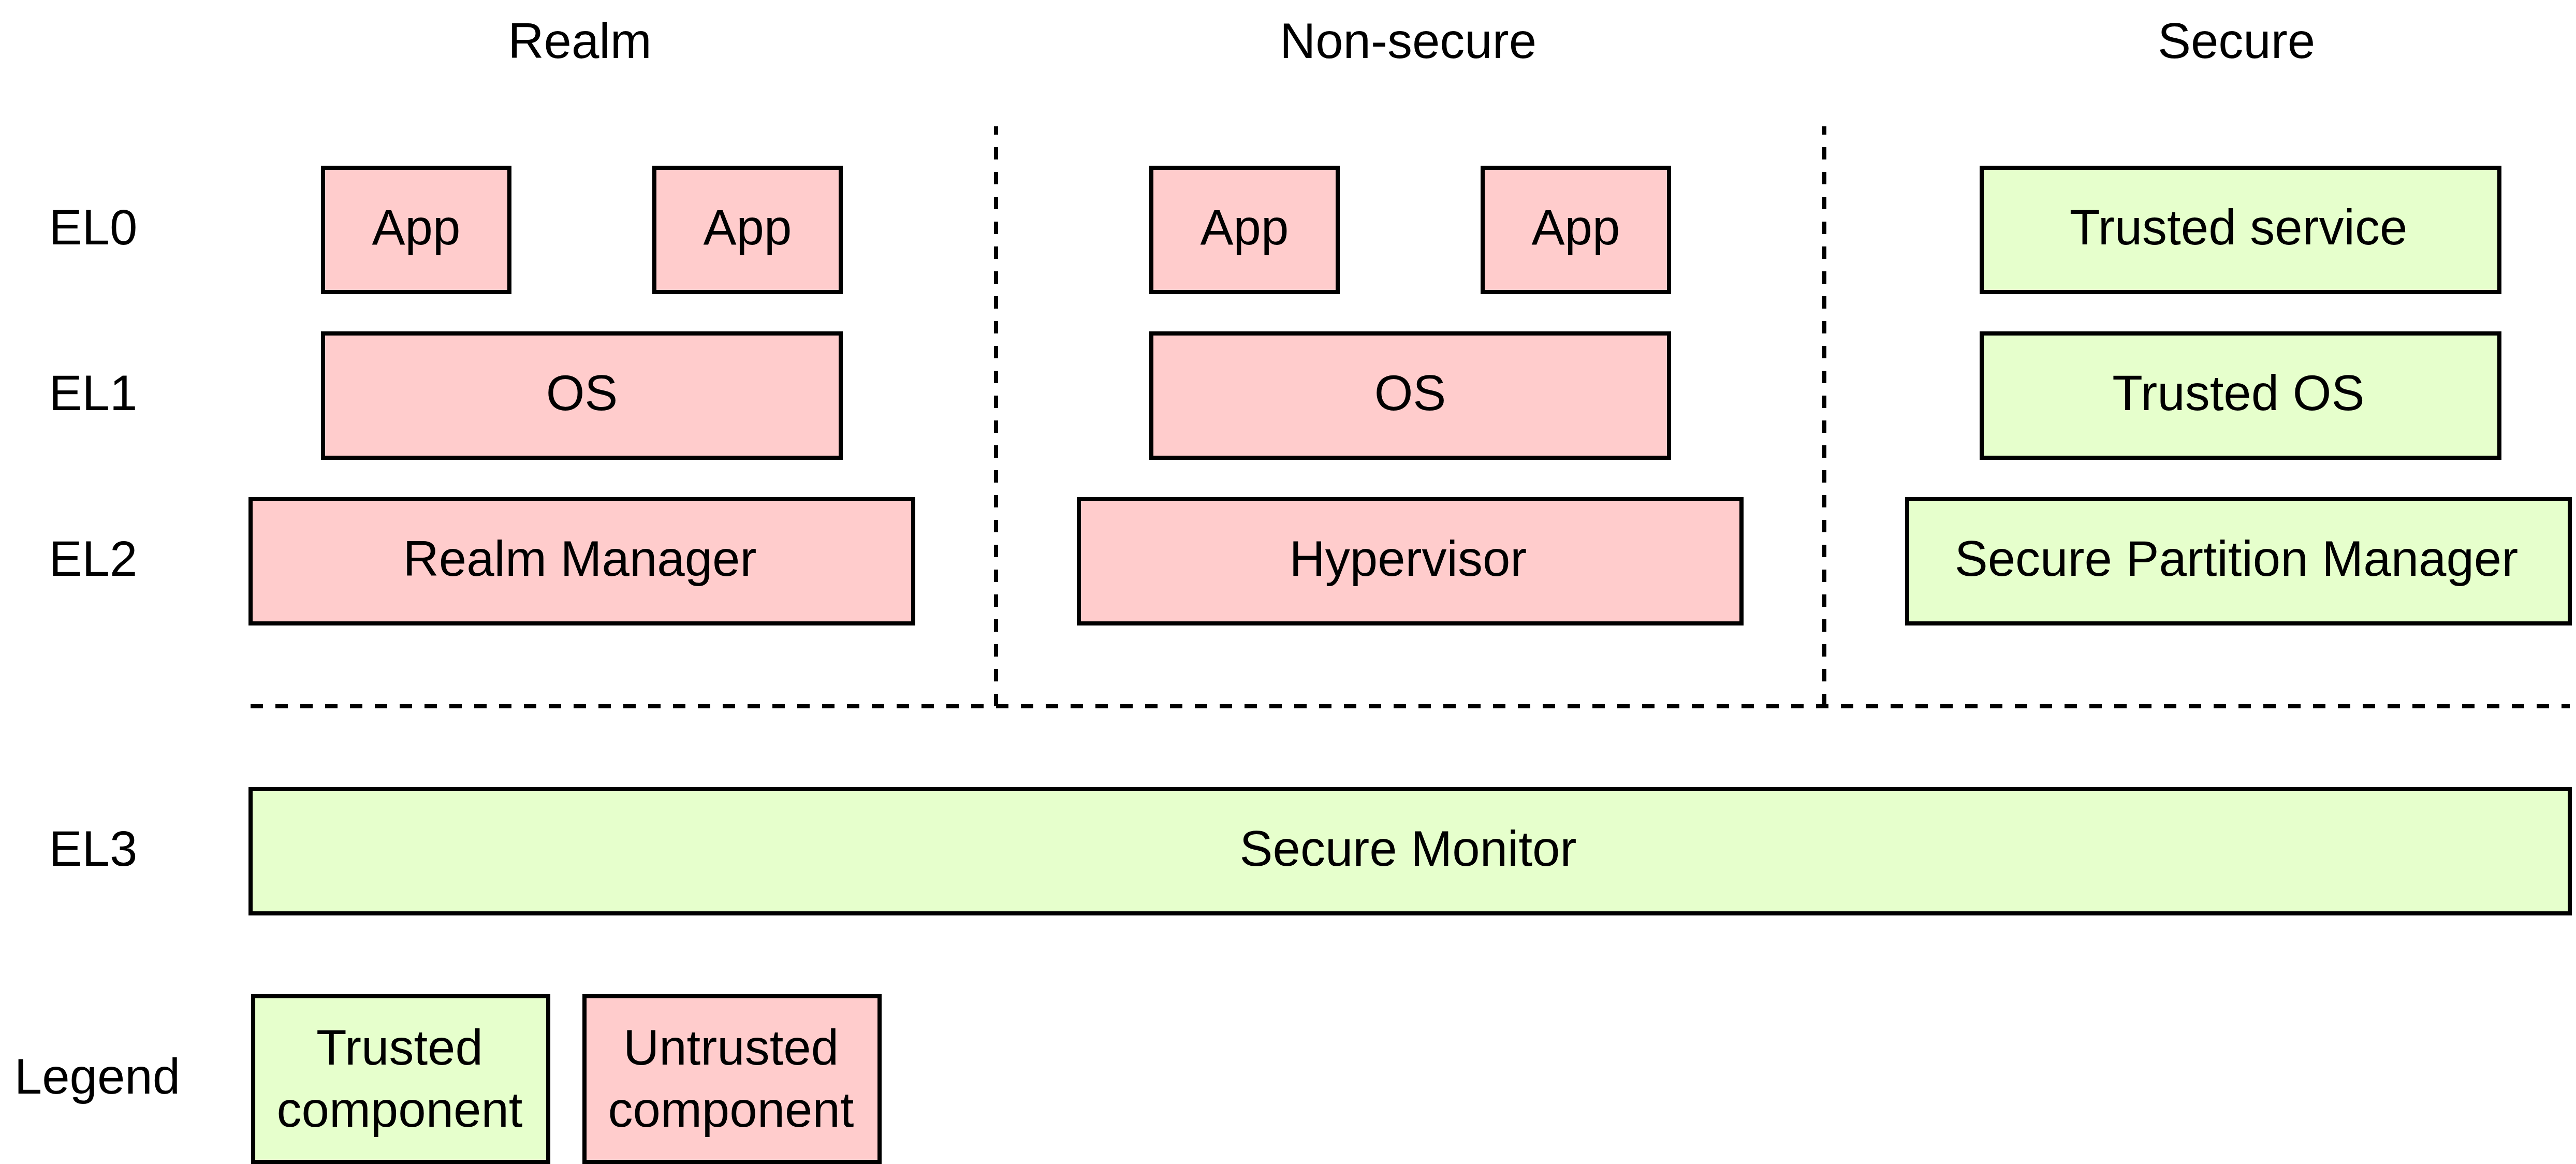
\includegraphics[width=\linewidth]{figures/armv9-cca}
\caption{ARMv9 Confidential Compute Architecture\label{fig:arm_cca}}
\end{figure}

Unlike AMD SEV-SNP or Intel TDX, which use dedicated CPU instructions to generate the attestation report, Arm TrustZone does not have a single
hardware instruction for attestation. Instead, it relies on a service-based model where the request is made through a Secure Monitor Call. In
traditional TrustZone environments, this is typically handled by a Trusted Execution Environment such as OP-TEE~\cite{op-tee_op-tee_nodate}, where a
specialized Trusted Application or the TEE kernel itself gathers measurements and signs them using hardware-fused keys. In the newer Arm CCA a
confidential "Realm" VM uses the Realm Service Interface to request an attestation token from the Realm Management Monitor firmware. While the
underlying hardware provides the isolation and keys, the actual report is generated by a firmware-level service like the logic found in OP-TEE or the
RMM.

\subsubsection{Intel}

The concept of encrypting secure application components in memory was first introduced in 2015 by Intel's Software Guard
Extensions~\cite{costan_intel_2016} with the Skylake architecture. This technology appeared in both server and client processors. SGX uses AES for
on-the-fly data encryption and decryption with a hardware-based encryption engine integrated into the CPU. The cryptographic keys used cannot be
exported from the processor. SGX introduced a new set of processor instructions that allow the creation of encrypted memory regions, known as
enclaves, within user-space processes. This method provides cryptographic protection for the enclave's data but requires applications to be split into
trusted and untrusted parts, making it costly for existing applications to adopt this approach, as they often need to be redesigned or rewritten.

In 2023, Intel released Trust Domain Extensions (TDX)~\cite{cheng_intel_2024} which allows deploying hardware-isolated virtual machines (VMs) called
trust domains (TDs). TD VMs are isolated from the virtual machine manager (VMM), hypervisor, and other software on the host platform. Intel TDX
combines several technologies, including virtual machine extensions (VMX), instruction-set-architecture (ISA) extensions, Intel Total Memory
Encryption Multi-key (Intel TME-MK), and CPU-attested software modules. The main component is the Intel TDX module, which is provided and digitally
signed by Intel. To host this module securely, but also to enforce security policies for TDs, a new SEcure Arbitration Mode -- SEAM mode of the CPU is
introduced. Figure~\ref{fig:intel_tdx} depicts Intel TDX architecture.

\begin{figure}[H]
\centering
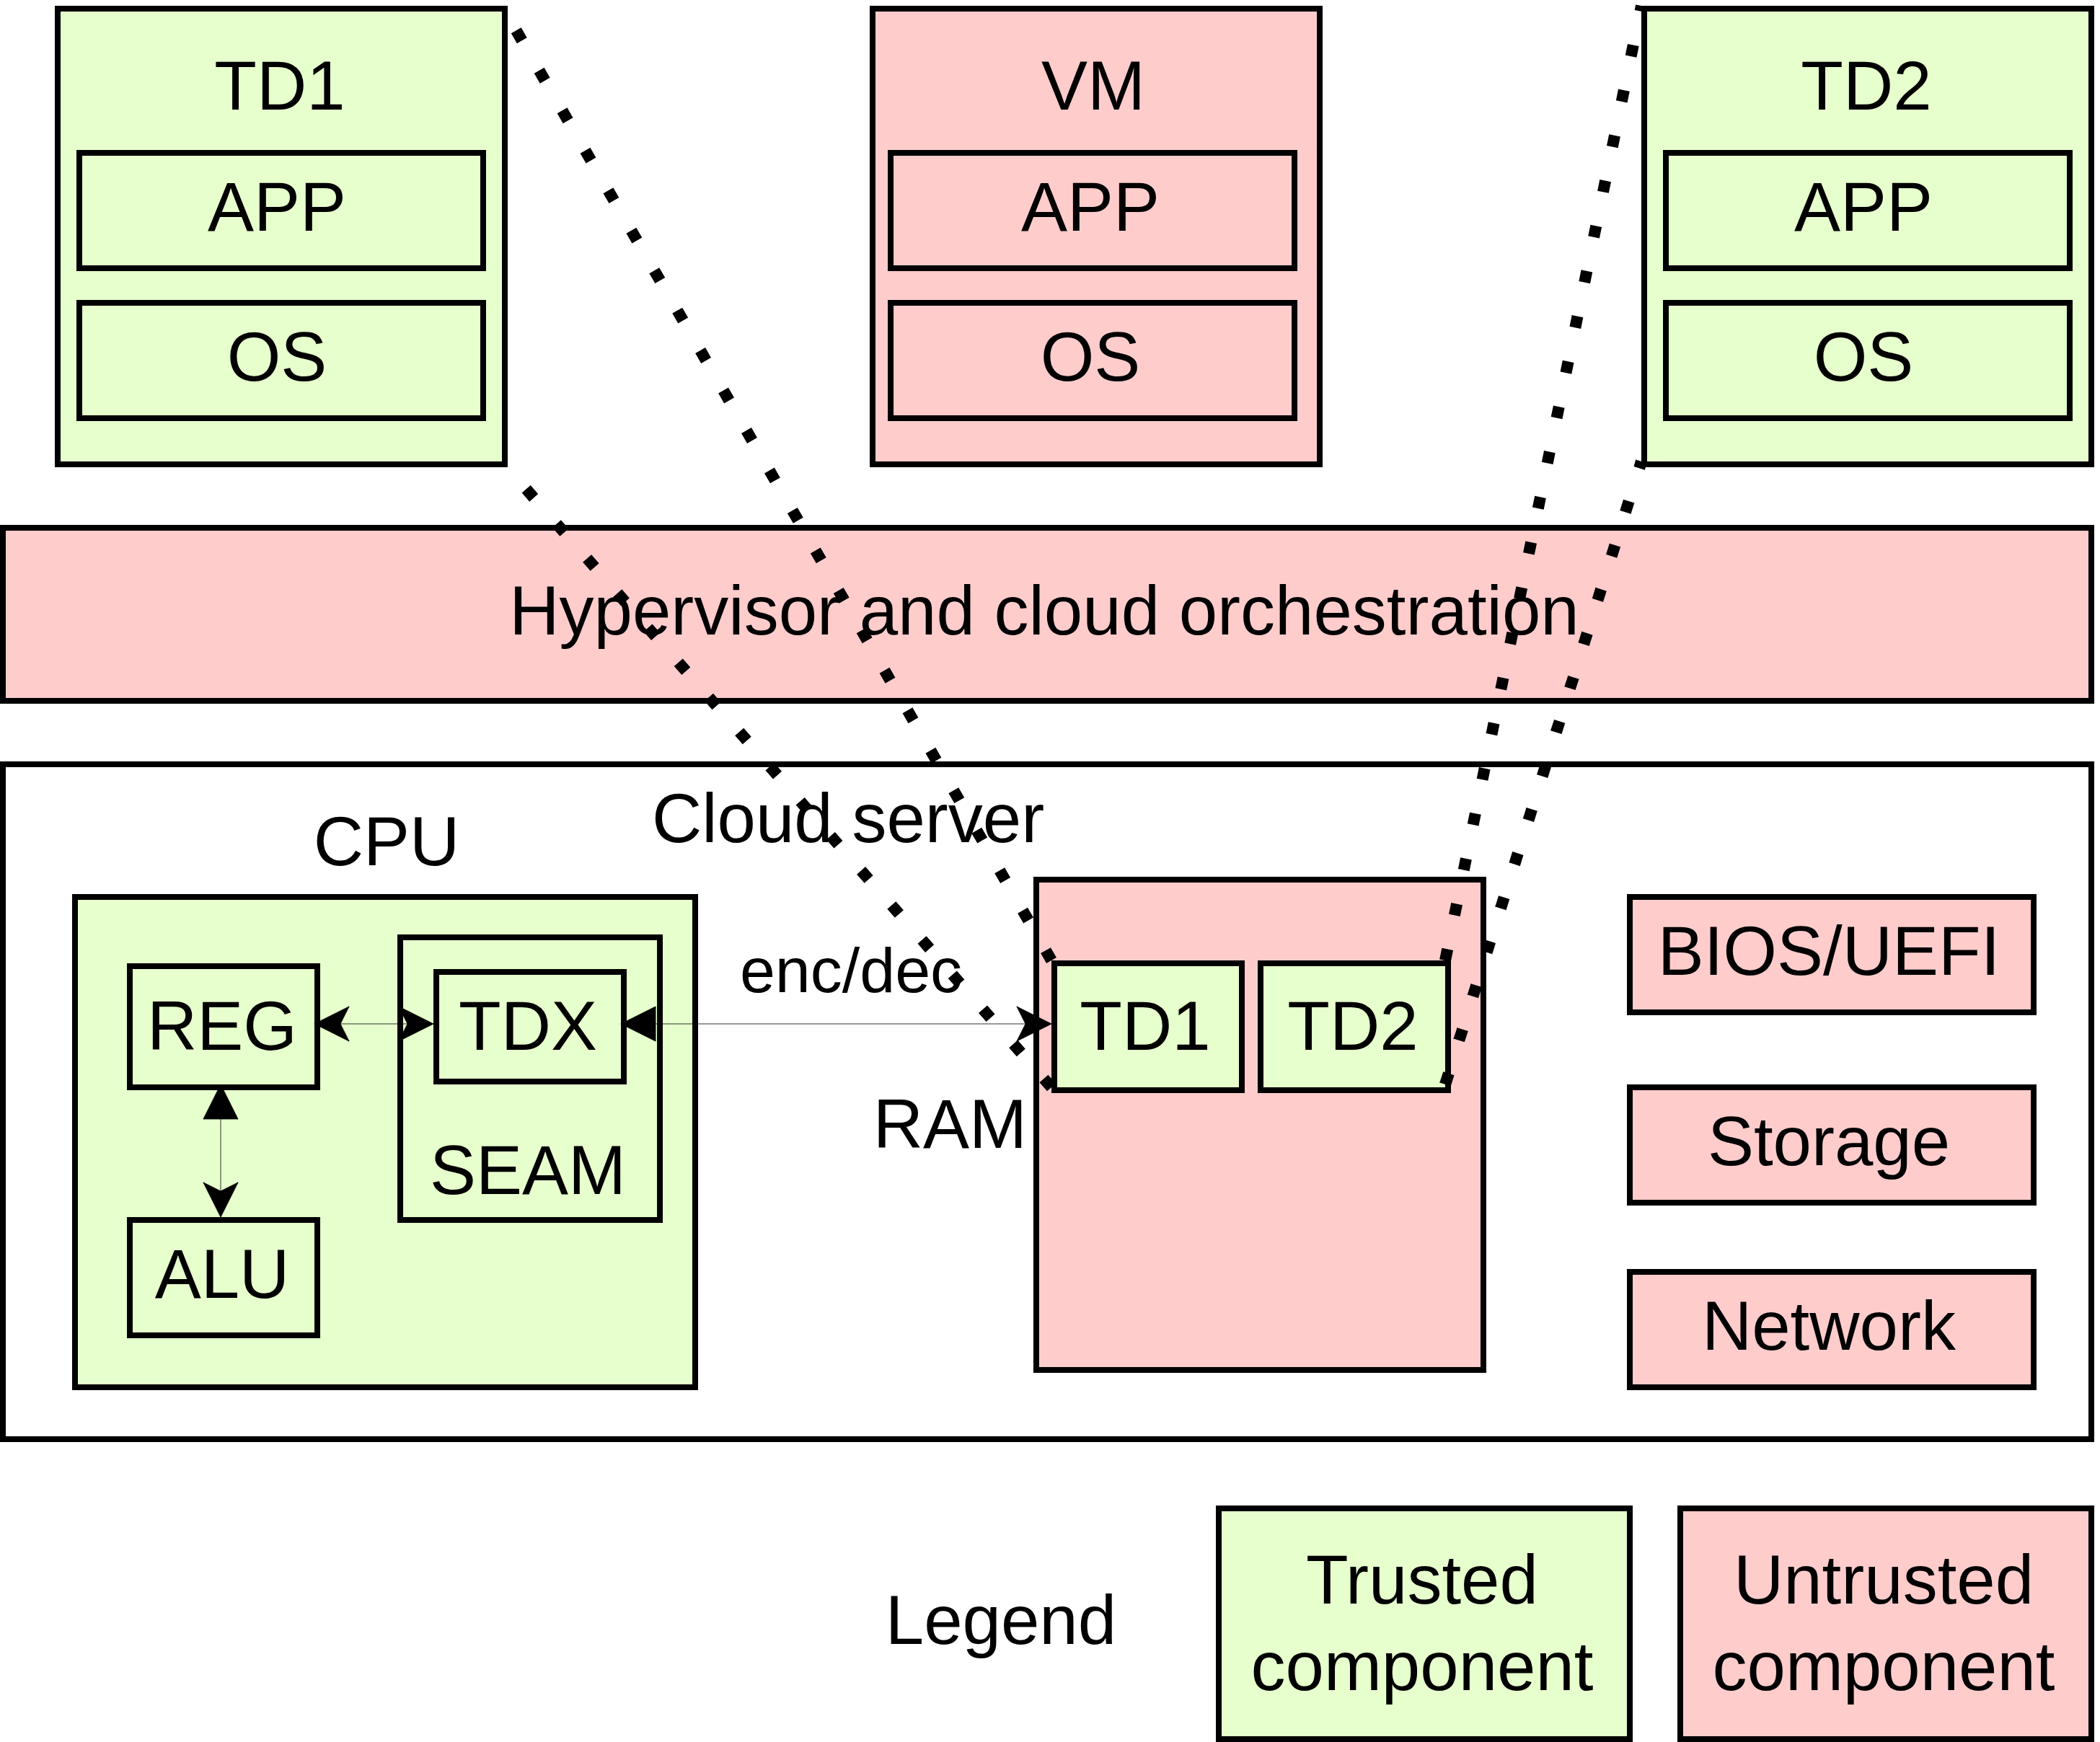
\includegraphics[width=10.5cm]{figures/intel-tdx}
\caption{High level architecture of the Intel TDX VM protection\label{fig:intel_tdx}}
\end{figure}

\subsubsection{AMD}

AMD Secure Encrypted Virtualisation (SEV) is designed to enhance the security of virtualised systems by encrypting the entire memory of a virtual
machine (VM). SEV works at the hypervisor and VM level, providing complete memory encryption for guest VMs. The AMD EPYC processors feature a
dedicated ARM-based Platform Secure Processor (PSP) that controls encryption and decryption with unique keys assigned to each VM, so that even if the
hypervisor is compromised, it is still unable to access the VM's contents. AMD has added extra capabilities to SEV, such as SEV-ES (Encrypted
State)~\cite{kaplan_protecting_2017} and SEV-SNP (Secure Nested Paging)~\cite{kaplan_amd_2020}, to maintain CPU register states securely and conduct
more rigorous memory integrity verification. Figure~\ref{fig:amd_sev} depicts AMD-SEV-SNP achitecture.

\begin{figure}[H]
\centering
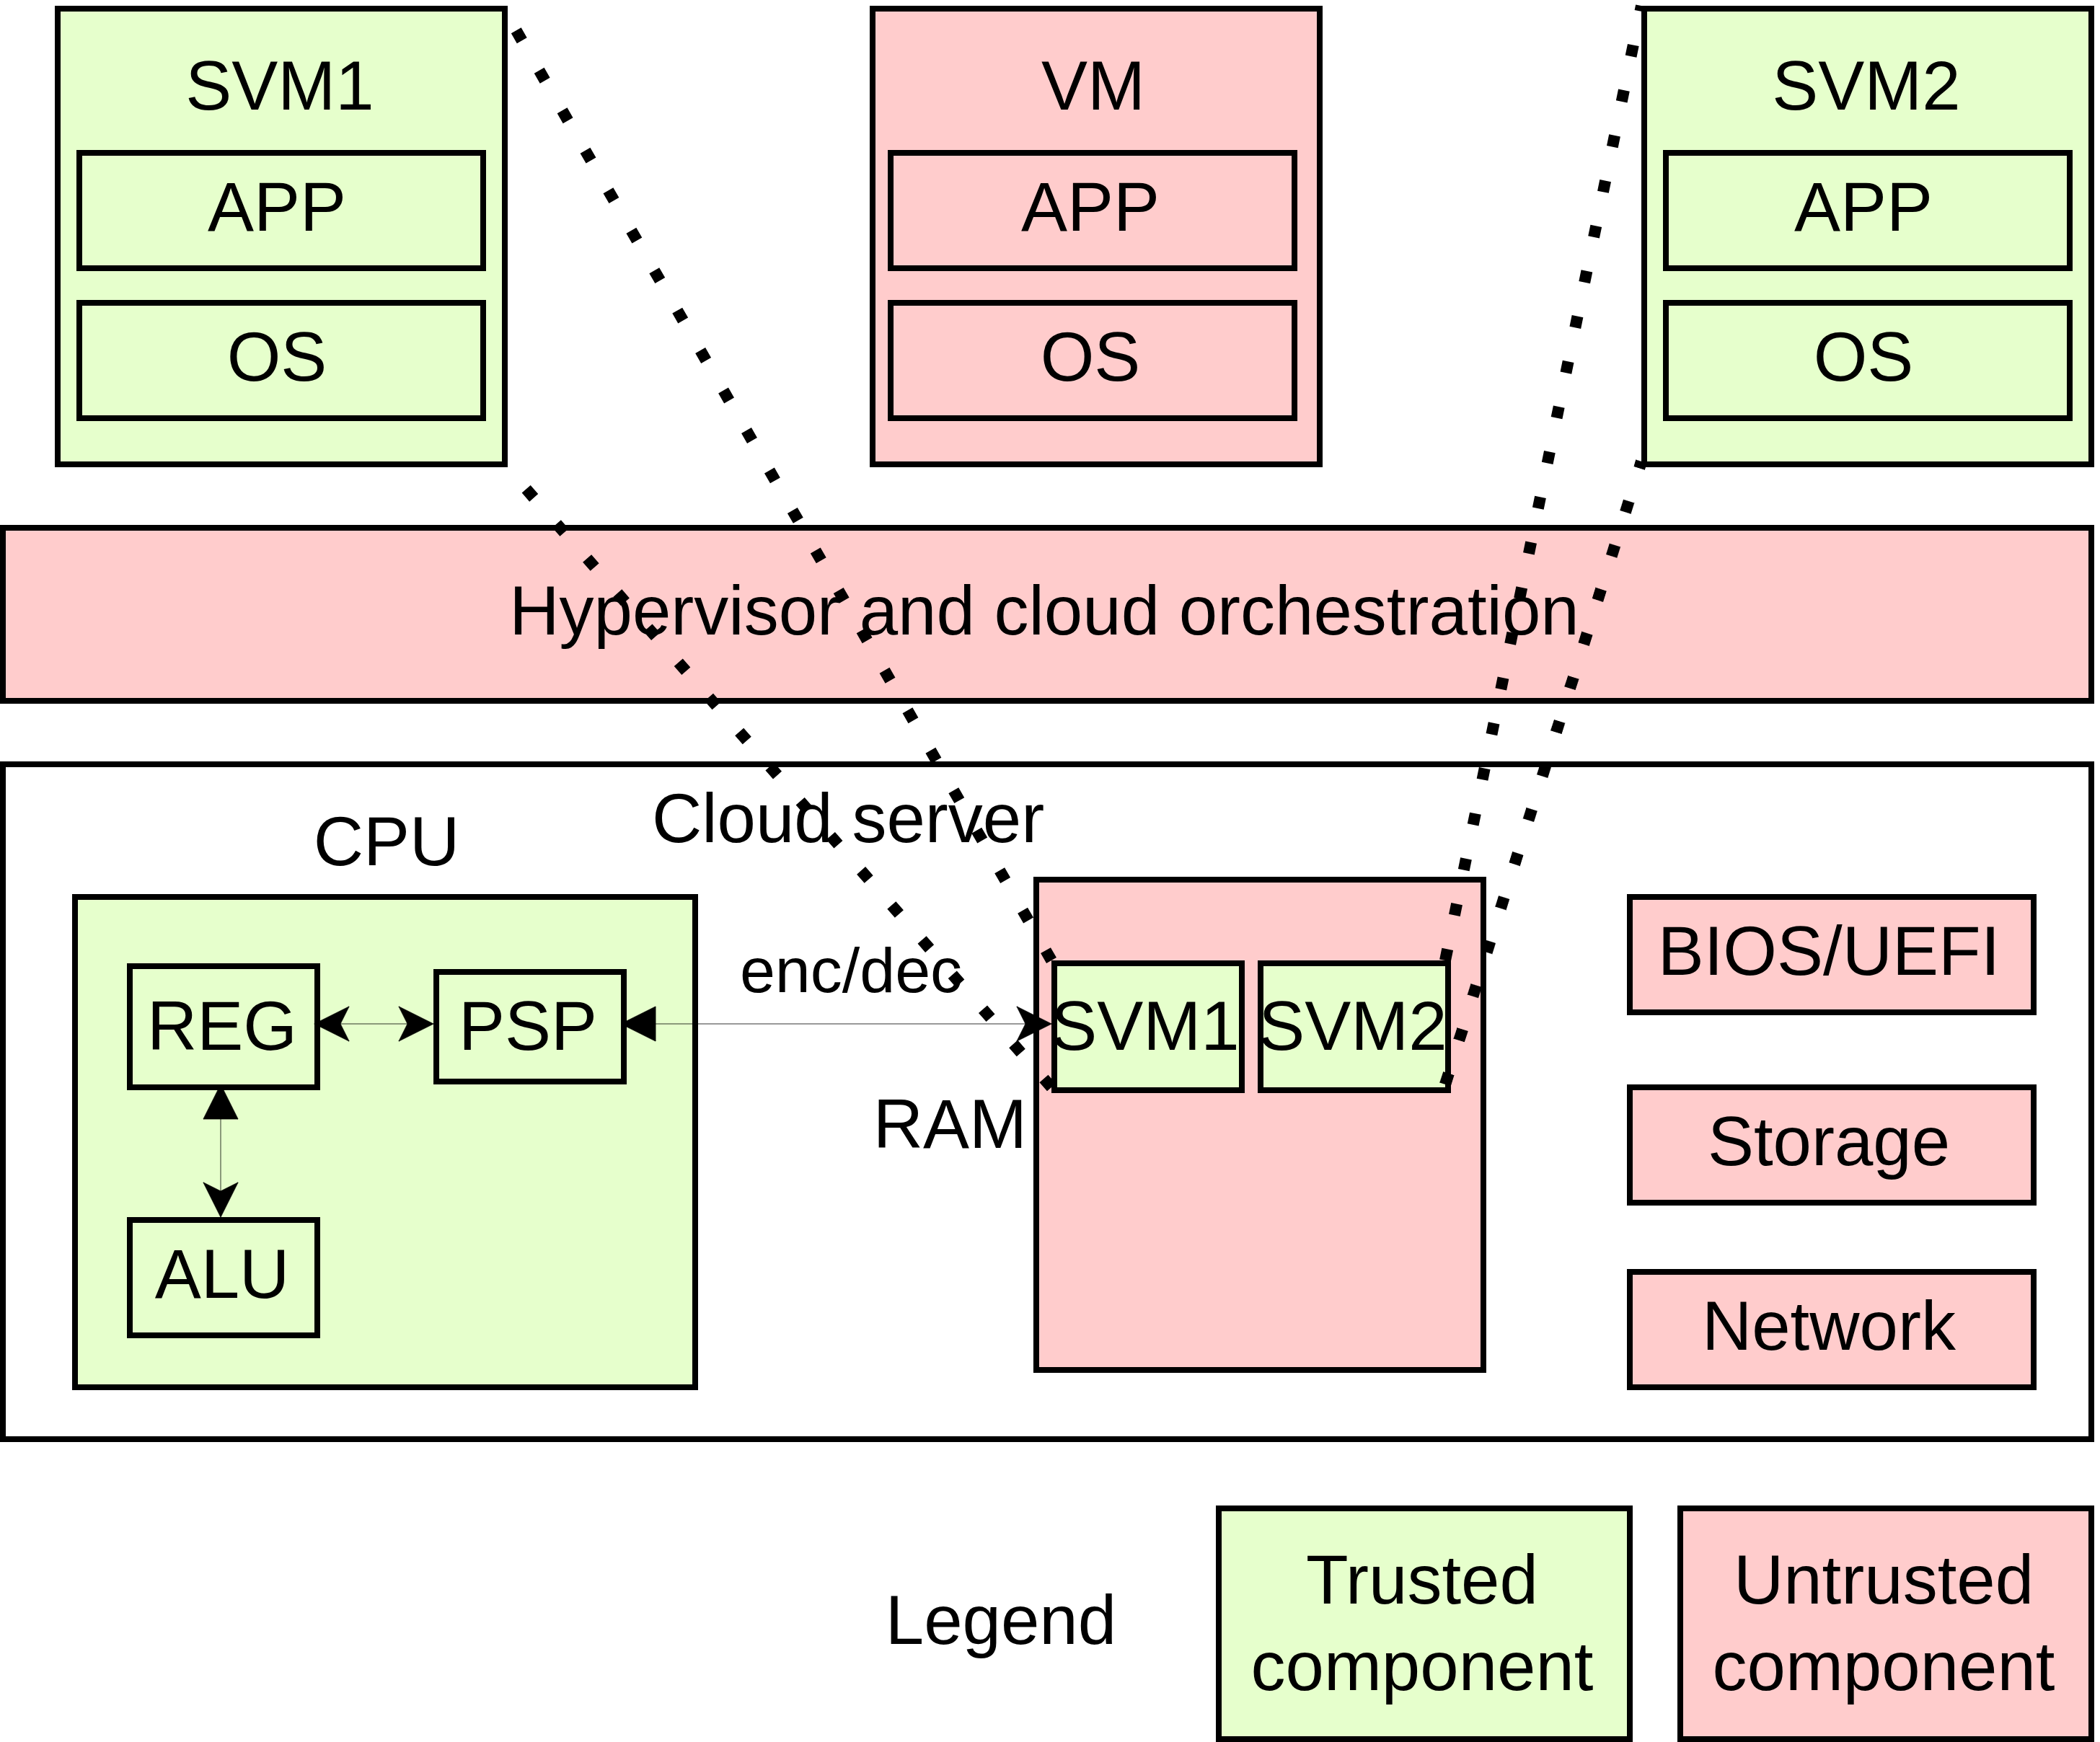
\includegraphics[width=10.5cm]{figures/amd-sev-snp}
\caption{High-level architecture of the AMD SEV VM protection\label{fig:amd_sev}}
\end{figure}

AMD's Secure Encrypted Virtualization (SEV) attestation has evolved from a complex, multi-party exchange in its first generations to a streamlined,
hardware-driven report system in the latest SEV-SNP (Secure Nested Paging) iteration.

\subsubsection{RISC-V}

RISC-V includes a well-defined privilege architecture. Most typical configuration defines three primary privilege levels: Machine mode (M-mode)
intended for firmware, Supervisor mode (S-mode) intended for the OS, and User mode (U-mode) intended for user applications. When the hypervisor RISC-V
extension is enabled four privilege levels are defined: Machine mode (M-mode) intended for firmware, Hypervisor-Extended Supervisor mode (HS-mode)
intended for the hypervisor, Virtual Supervisor mode (VS-mode) intended for the guest OS and Virtualized User mode (VU-mode) intended for guest user
applications. Machine mode has the highest level of control and is responsible for low-level hardware management. These privilege levels are depicted
in Figure~\ref{fig:riscv_privilege_modes}.

\begin{figure}[H]
\centering
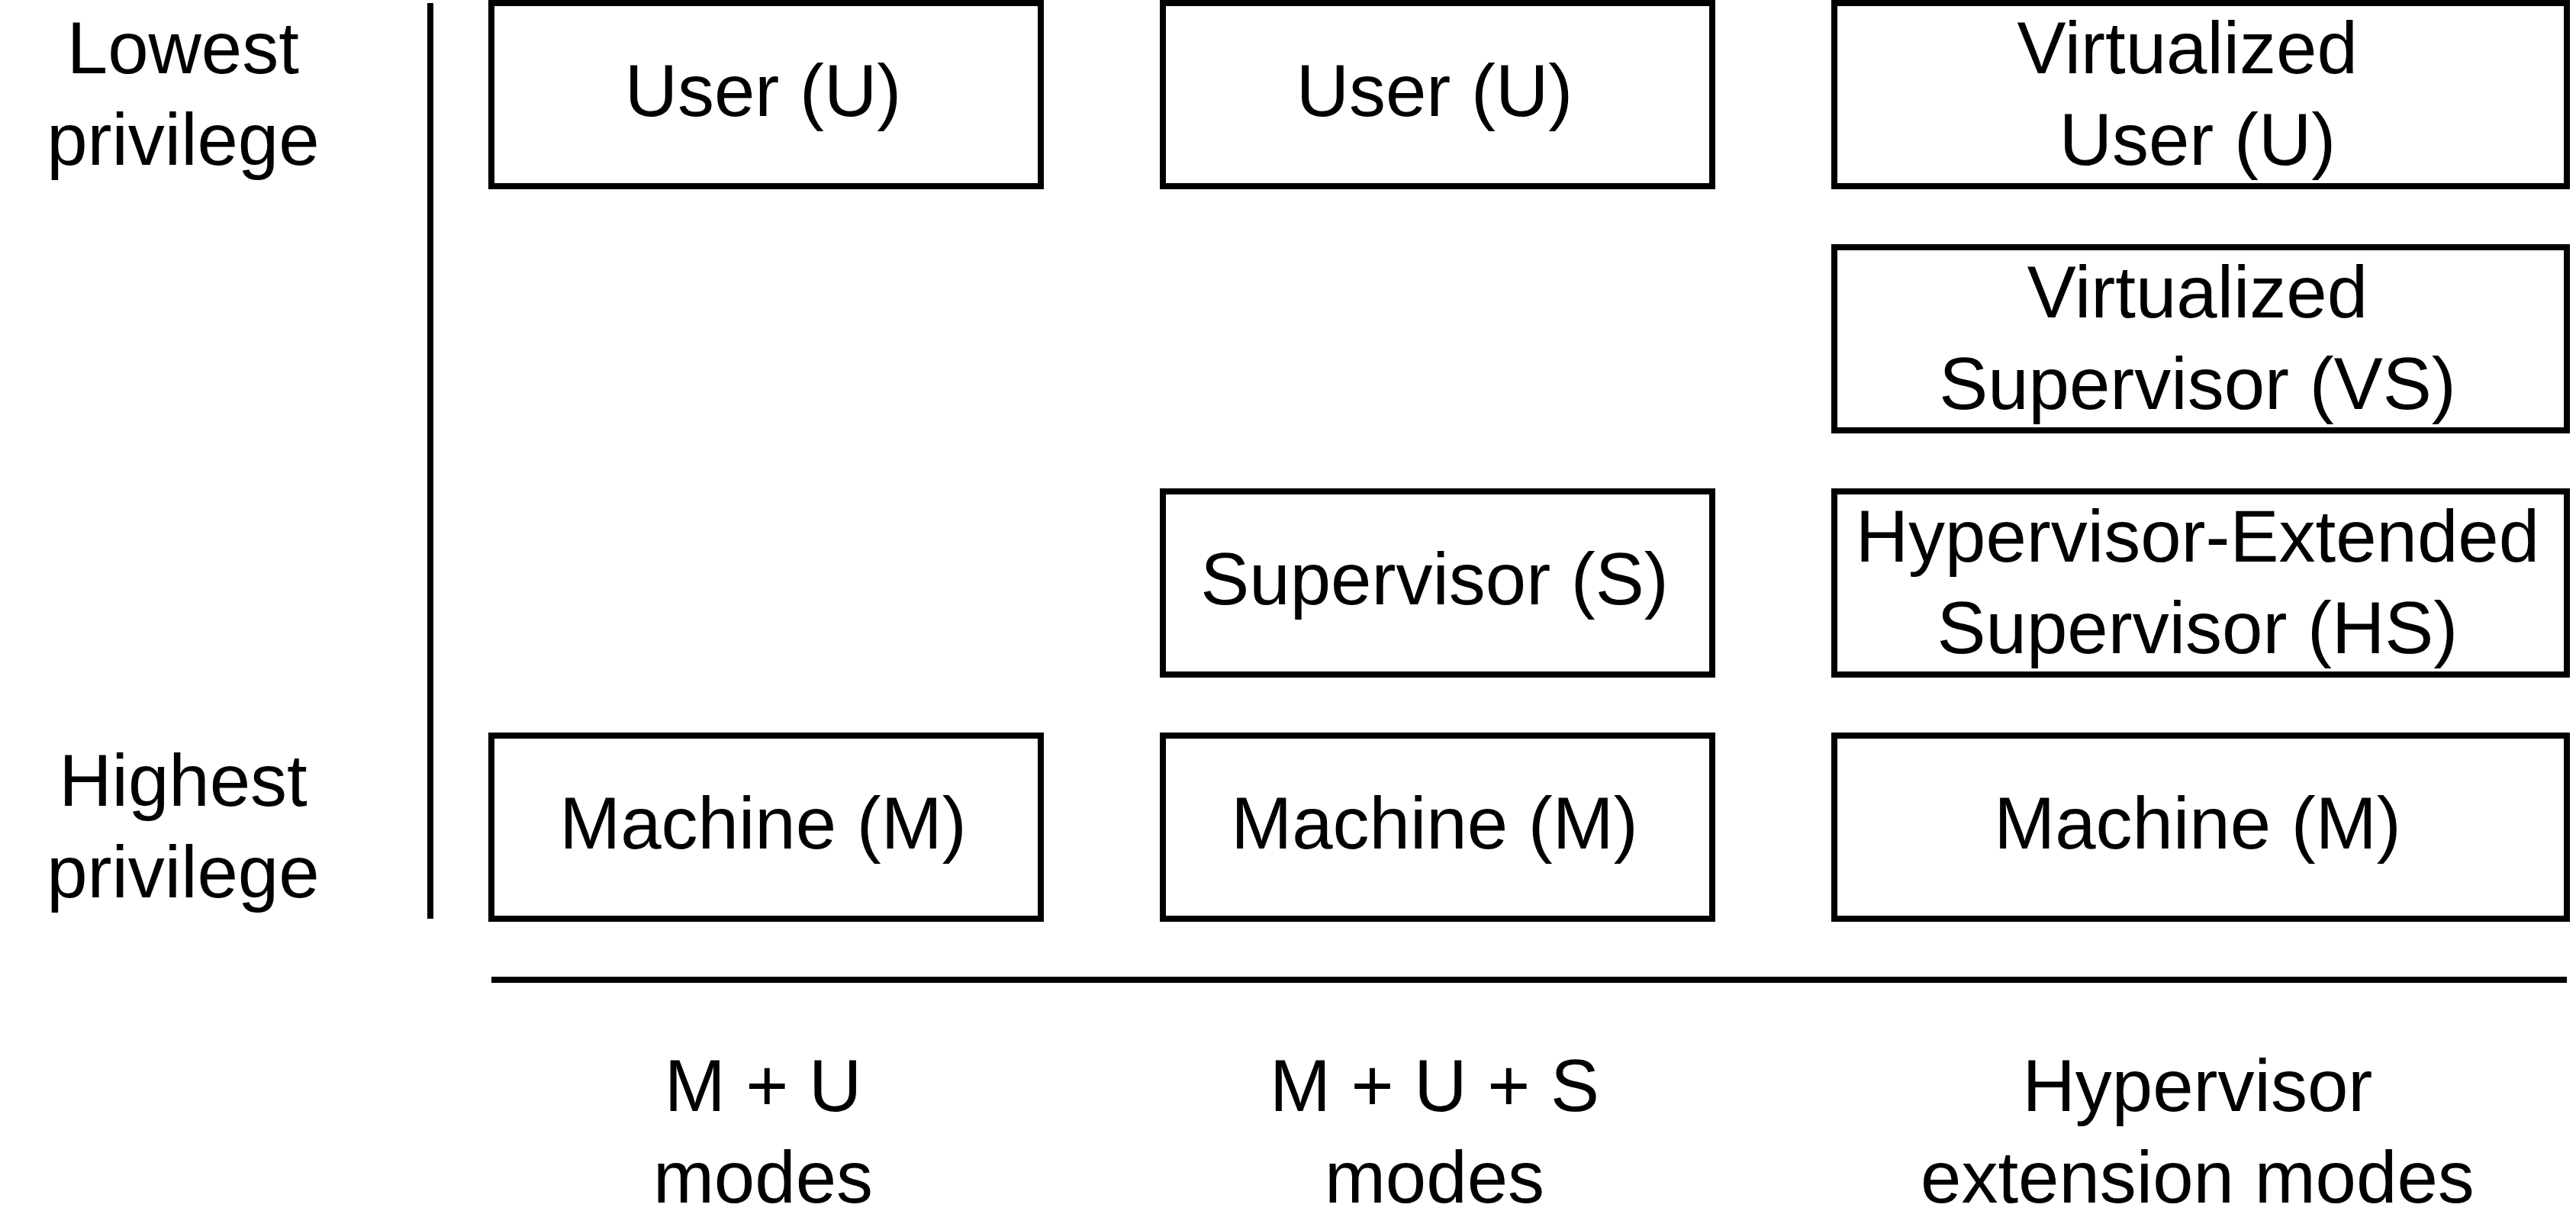
\includegraphics[width=11.3cm]{figures/riscv-privilege-modes}
\caption{RISC-V privilege modes\label{fig:riscv_privilege_modes}}
\end{figure}

An important security feature within this architecture is the Physical Memory Protection (PMP)~\cite{waterman_risc-v_2016} system. PMP is a hardware
mechanism that enables fine-grained memory isolation and controls access to physical memory regions based on privilege level and access type. These
rules are configured through special control and status registers (CSRs), only accessible in Machine mode. Each PMP entry defines a region of memory
and associated permissions, and multiple entries can be configured to create a comprehensive protection policy. The process of enforcing PMP rules is
depicted in Figure~\ref{fig:riscv_pmp}.

\begin{figure}[H]
\centering
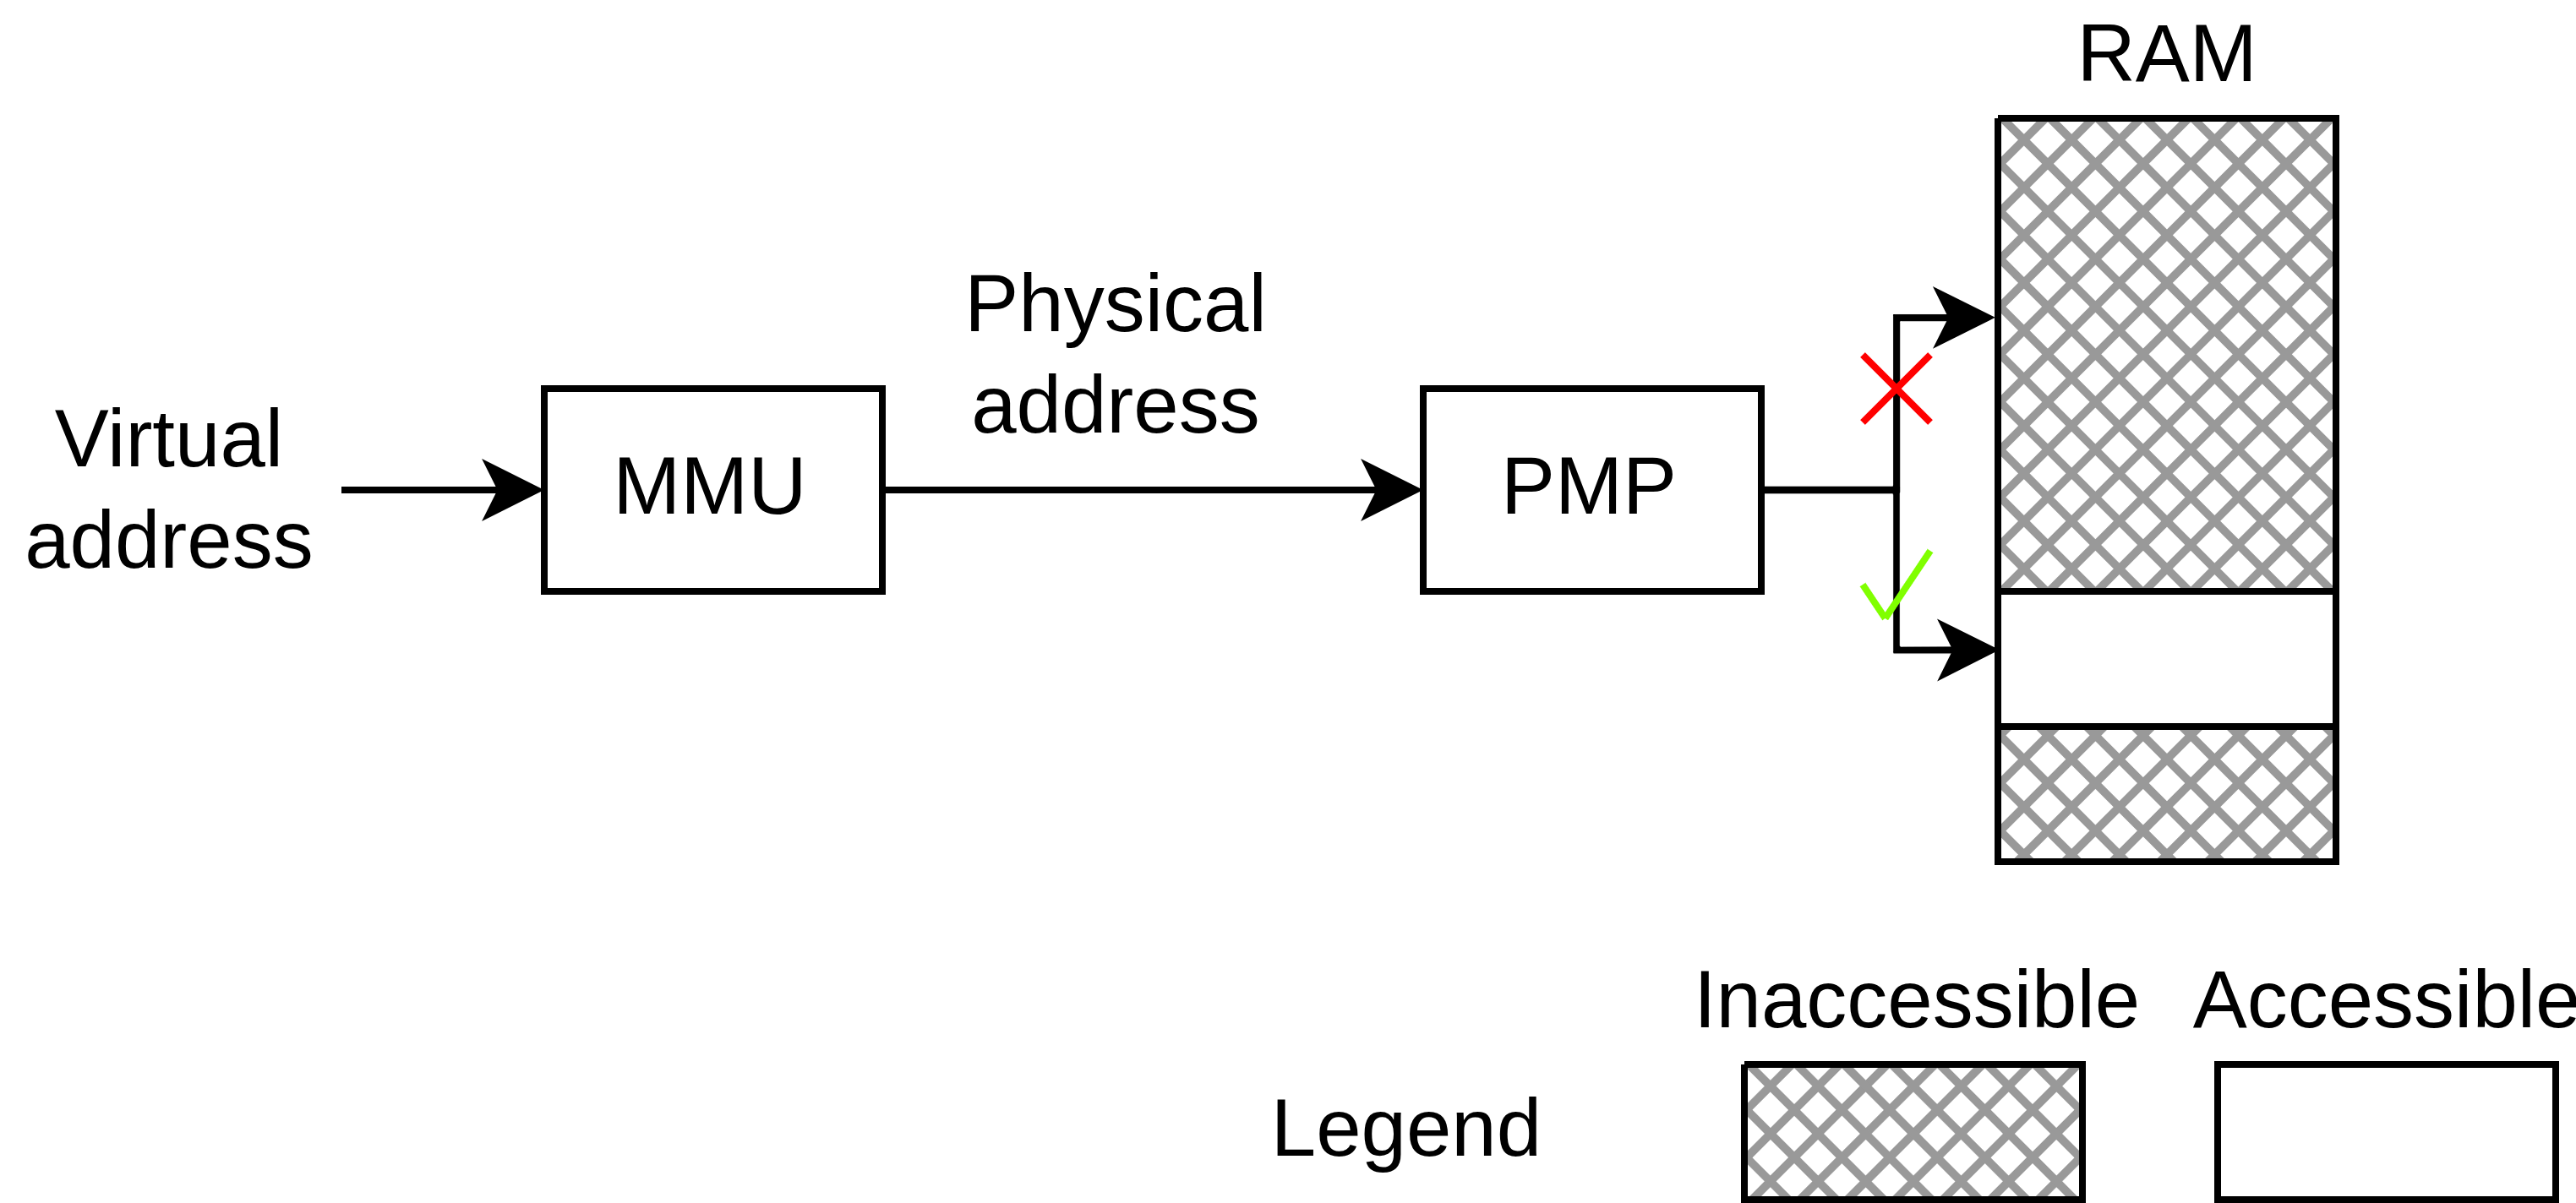
\includegraphics[width=9.2cm]{figures/riscv-pmp}
\caption{RISC-V PMP\label{fig:riscv_pmp}}
\end{figure}

Physical Memory Protection (PMP) mechanism itself does not include support for memory encryption. To the authors' best knowledge, the RISC-V
Application Platform - Trusted Execution Environment Task Group (AP-TEE TG) doesn't currently provide memory encryption as ratified extension. If
memory encryption is required, hardware manufacturers must integrate a dedicated memory encryption engine into the system. A proposal on how to
achieve this is described in~\cite{moolman_extending_2024}.

Unlike Intel or AMD, RISC-V provides basic capabilities that serve as a foundation for more advanced security frameworks such as
Keystone~\cite{lee_keystone_2019}, CoVE~\cite{sahita_cove_2023} and IBM ACE~\cite{ozga_ace_2025}. These platforms aim to deliver functionality
comparable to trusted execution environments like Intel SGX, Intel TDX, and AMD SEV. A more in-depth analysis of the available RISC-V platforms is
available in~\cite{boubakri_survey_2025}.

Similar to ARM TrustZone, attestation is not implemented as a fixed, hardwired hardware primitive. Instead, the architecture provides the foundational
isolation and privilege mechanisms, while the concrete attestation protocol is typically realized in software that is running in M-mode. In the
Keystone framework, which this paper builds upon, the attestation mechanism is integrated into the Security Monitor. The Security Monitor
runs in M-mode and is responsible for enclave lifecycle management, isolation enforcement, and measurement. As part of the attestation process, it
generates cryptographic reports that reflect the identity and integrity of an enclave. Because the Security Monitor operates at the highest privilege
level, it can securely access hardware features such as Physical Memory Protection (PMP) and device-specific keys, allowing it to produce trustworthy
attestation evidence for remote verification.

\subsubsection{Summary}

Table~\ref{tab:tee_summary} provides a summary of TEE platforms described in the previous chapters. The summary focuses on five properties: isolated
execution, software authenticity, runtime integrity, data/storage confidentiality, and remote attestation.

\begin{table}[H]
\caption{TEE summary.\label{tab:tee_summary}}
\begin{adjustwidth}{-\extralength}{0cm}
\small
\newcolumntype{L}{>{\raggedright\arraybackslash}X}
\begin{tabularx}{\fulllength}{%
  >{\raggedright\arraybackslash}p{3.2cm}>{\centering\arraybackslash}p{1.8cm}>{\centering\arraybackslash}p{1.9cm}%
  LL>{\centering\arraybackslash}p{1.8cm}}
\toprule
\textbf{Platform} & \textbf{Isolated Execution} & \textbf{Software Authenticity} & \textbf{Runtime Integrity} & \textbf{Data/Storage Confidentiality}
& \textbf{Remote Attestation}\\
\midrule
Arm TrustZone/CCA & Yes & Yes & Partial to strong, depending on variant & Partial in classic TrustZone; stronger in CCA & Yes\\
Intel SGX/TDX & Yes & Yes & Strong & Strong & Yes\\
AMD SEV/SEV-ES/SEV-SNP & Yes & Yes & Strongest in SEV-SNP; SEV-ES protects CPU register state; SEV-SNP adds integrity protection against malicious
hypervisor memory manipulation & Strong & Yes\\
RISC-V (Keystone/CoVE-style) & Yes & Yes & Moderate to strong, platform-dependent & Moderate by default & Yes\\
\bottomrule
\end{tabularx}
\end{adjustwidth}
\end{table}

Arm, Intel, AMD, and RISC-V all support isolated execution and attestation, but they differ significantly in granularity and confidentiality model:
Arm historically emphasizes secure-world separation, Intel spans enclave and VM-level TEEs, AMD focuses on encrypted confidential VMs, while RISC-V
currently relies more on open architectural isolation primitives and monitor-based designs, with memory encryption still largely platform-specific
rather than standardized.

%%%%%%%%%%%%%%%%%%%%%
\section{QTEE-V Architecture}

The system presented in this study aims to solve the problem of the limited range of QKD systems by introducing trusted relay nodes between the QKD
links on a path between two endpoints. The overall architecture of the proposed system is given in Figure~\ref{fig:architecture}. It is similar to
standardized QKD network setups, with the key difference which is the use of the principles and methods of confidential computing on \emph{secure
relays} built on open architecture to further strengthen end-to-end key security.

\begin{figure}[H]
\centering
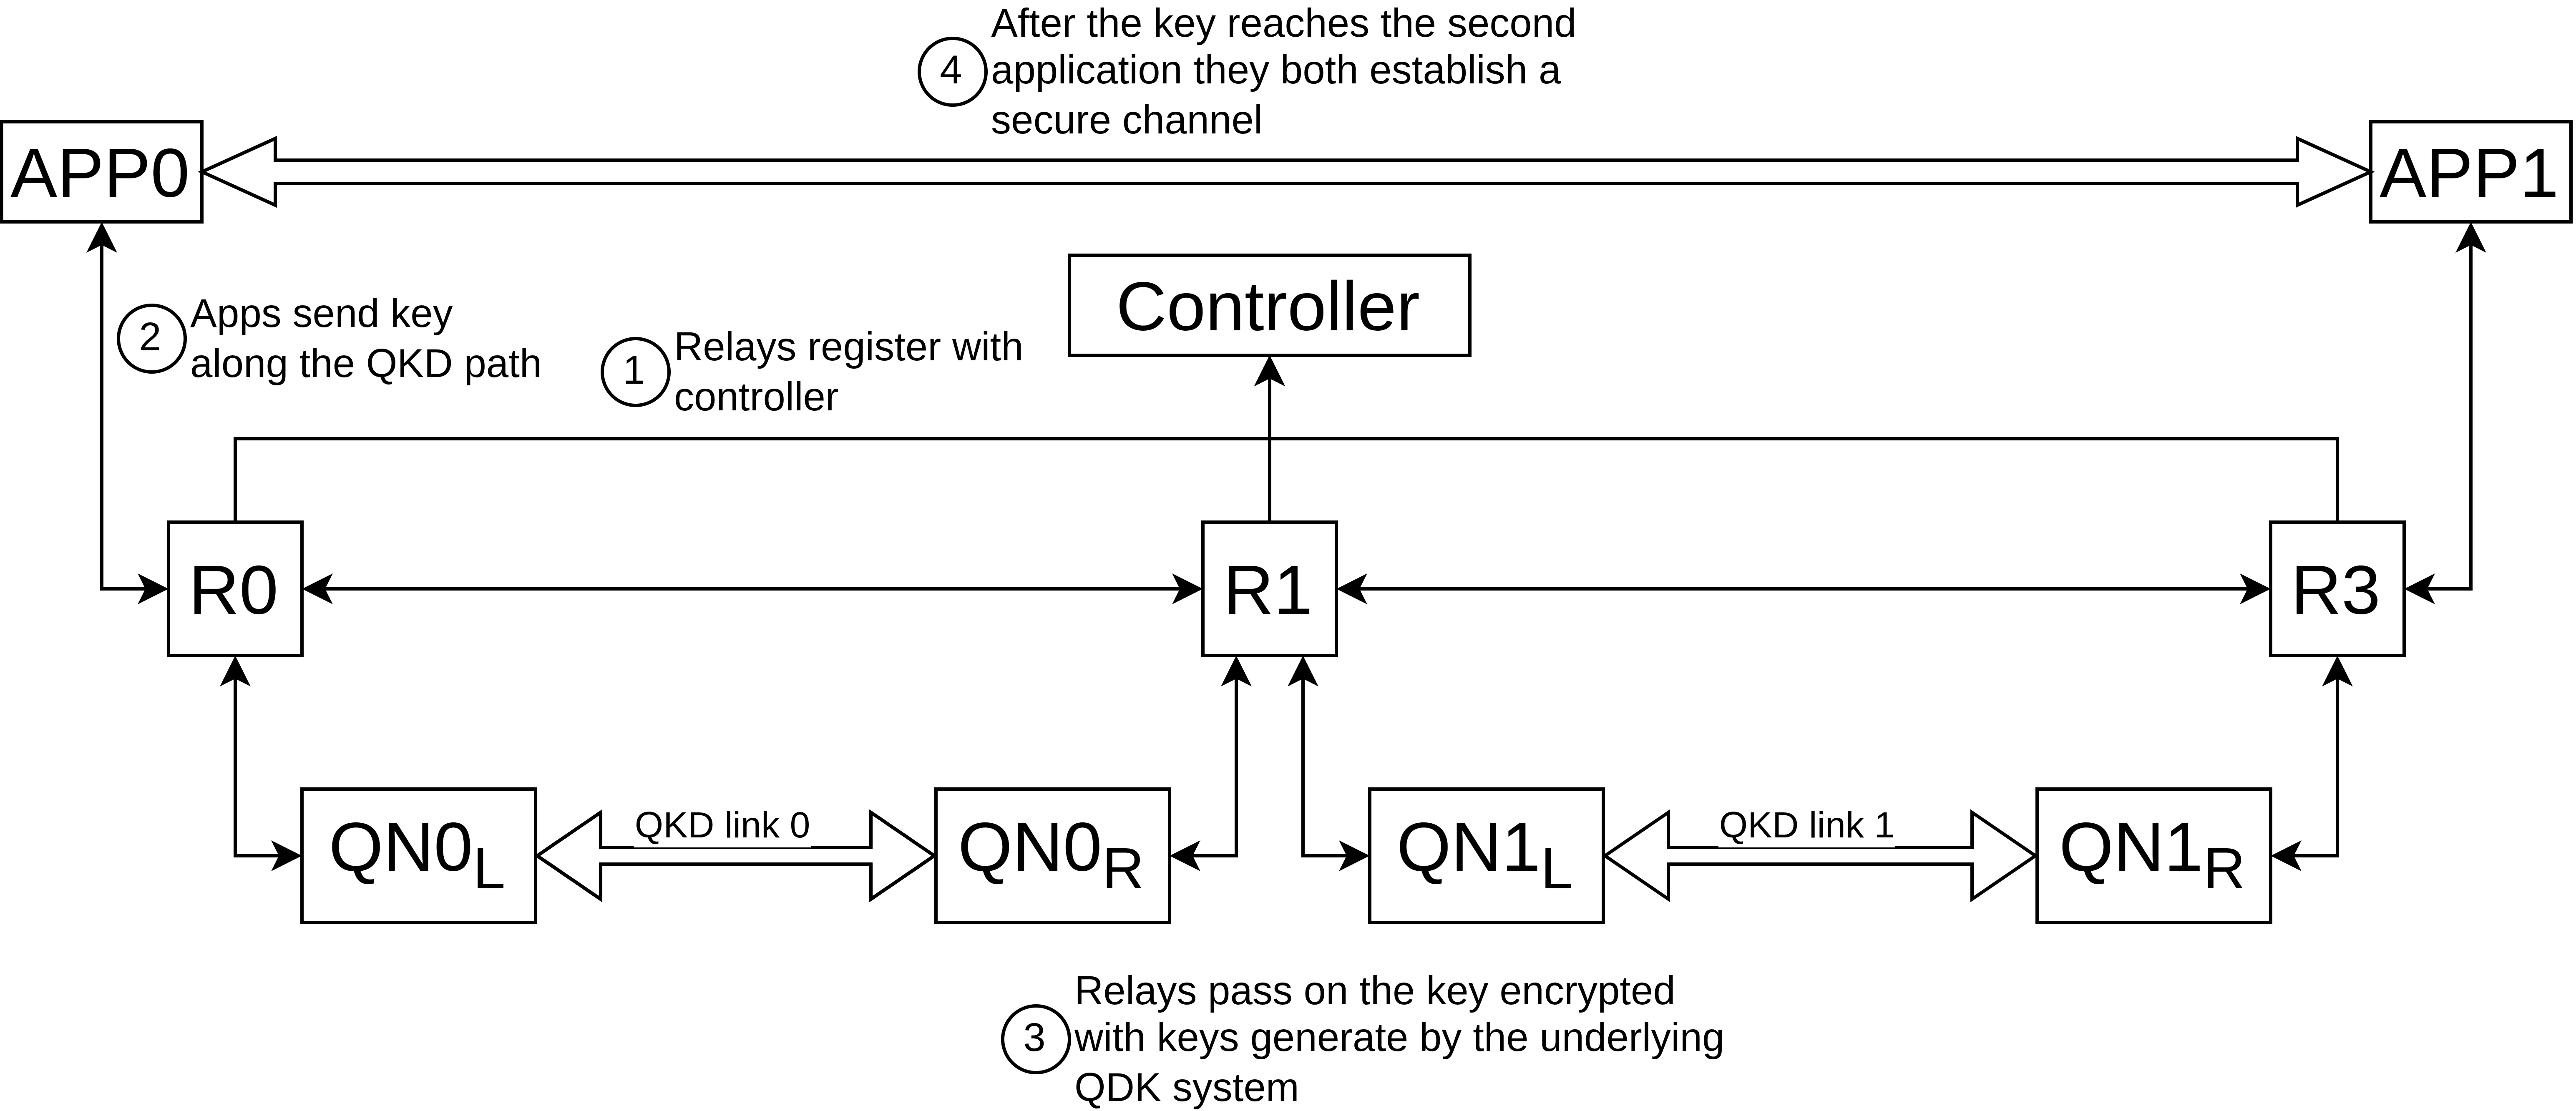
\includegraphics[width=\linewidth]{figures/architecture}
\caption{Architecture of the system\label{fig:architecture}}
\end{figure}

The system consists of several components:

\begin{itemize}
\item QKD nodes and links responsible for generating and transferring keys for relays (denoted with QN0\textsubscript{L}, QN0\textsubscript{R},
QN1\textsubscript{L} and QN1\textsubscript{R}).One pair of nodes forms a QKD link (QKD link 0 and QKD link 1);
\item Secure relays running inside a RISC-V TEE enclaves (denoted with R0, R1 and R2);
\item Applications that exchange keys using the proposed system (denoted with APP0 and APP1);
\item Central controller;
\end{itemize}

The key components, their role in the system and how they communicate with each other are described in subsequent sections.

\subsection{QKD Link}

The long-distance QKD path consists of more than one QKD links. Each link has two QKD nodes at its ends. Figure~\ref{fig:qkd_link} depicts one QKD
link with the accompanying components.

\begin{figure}[H]
\centering
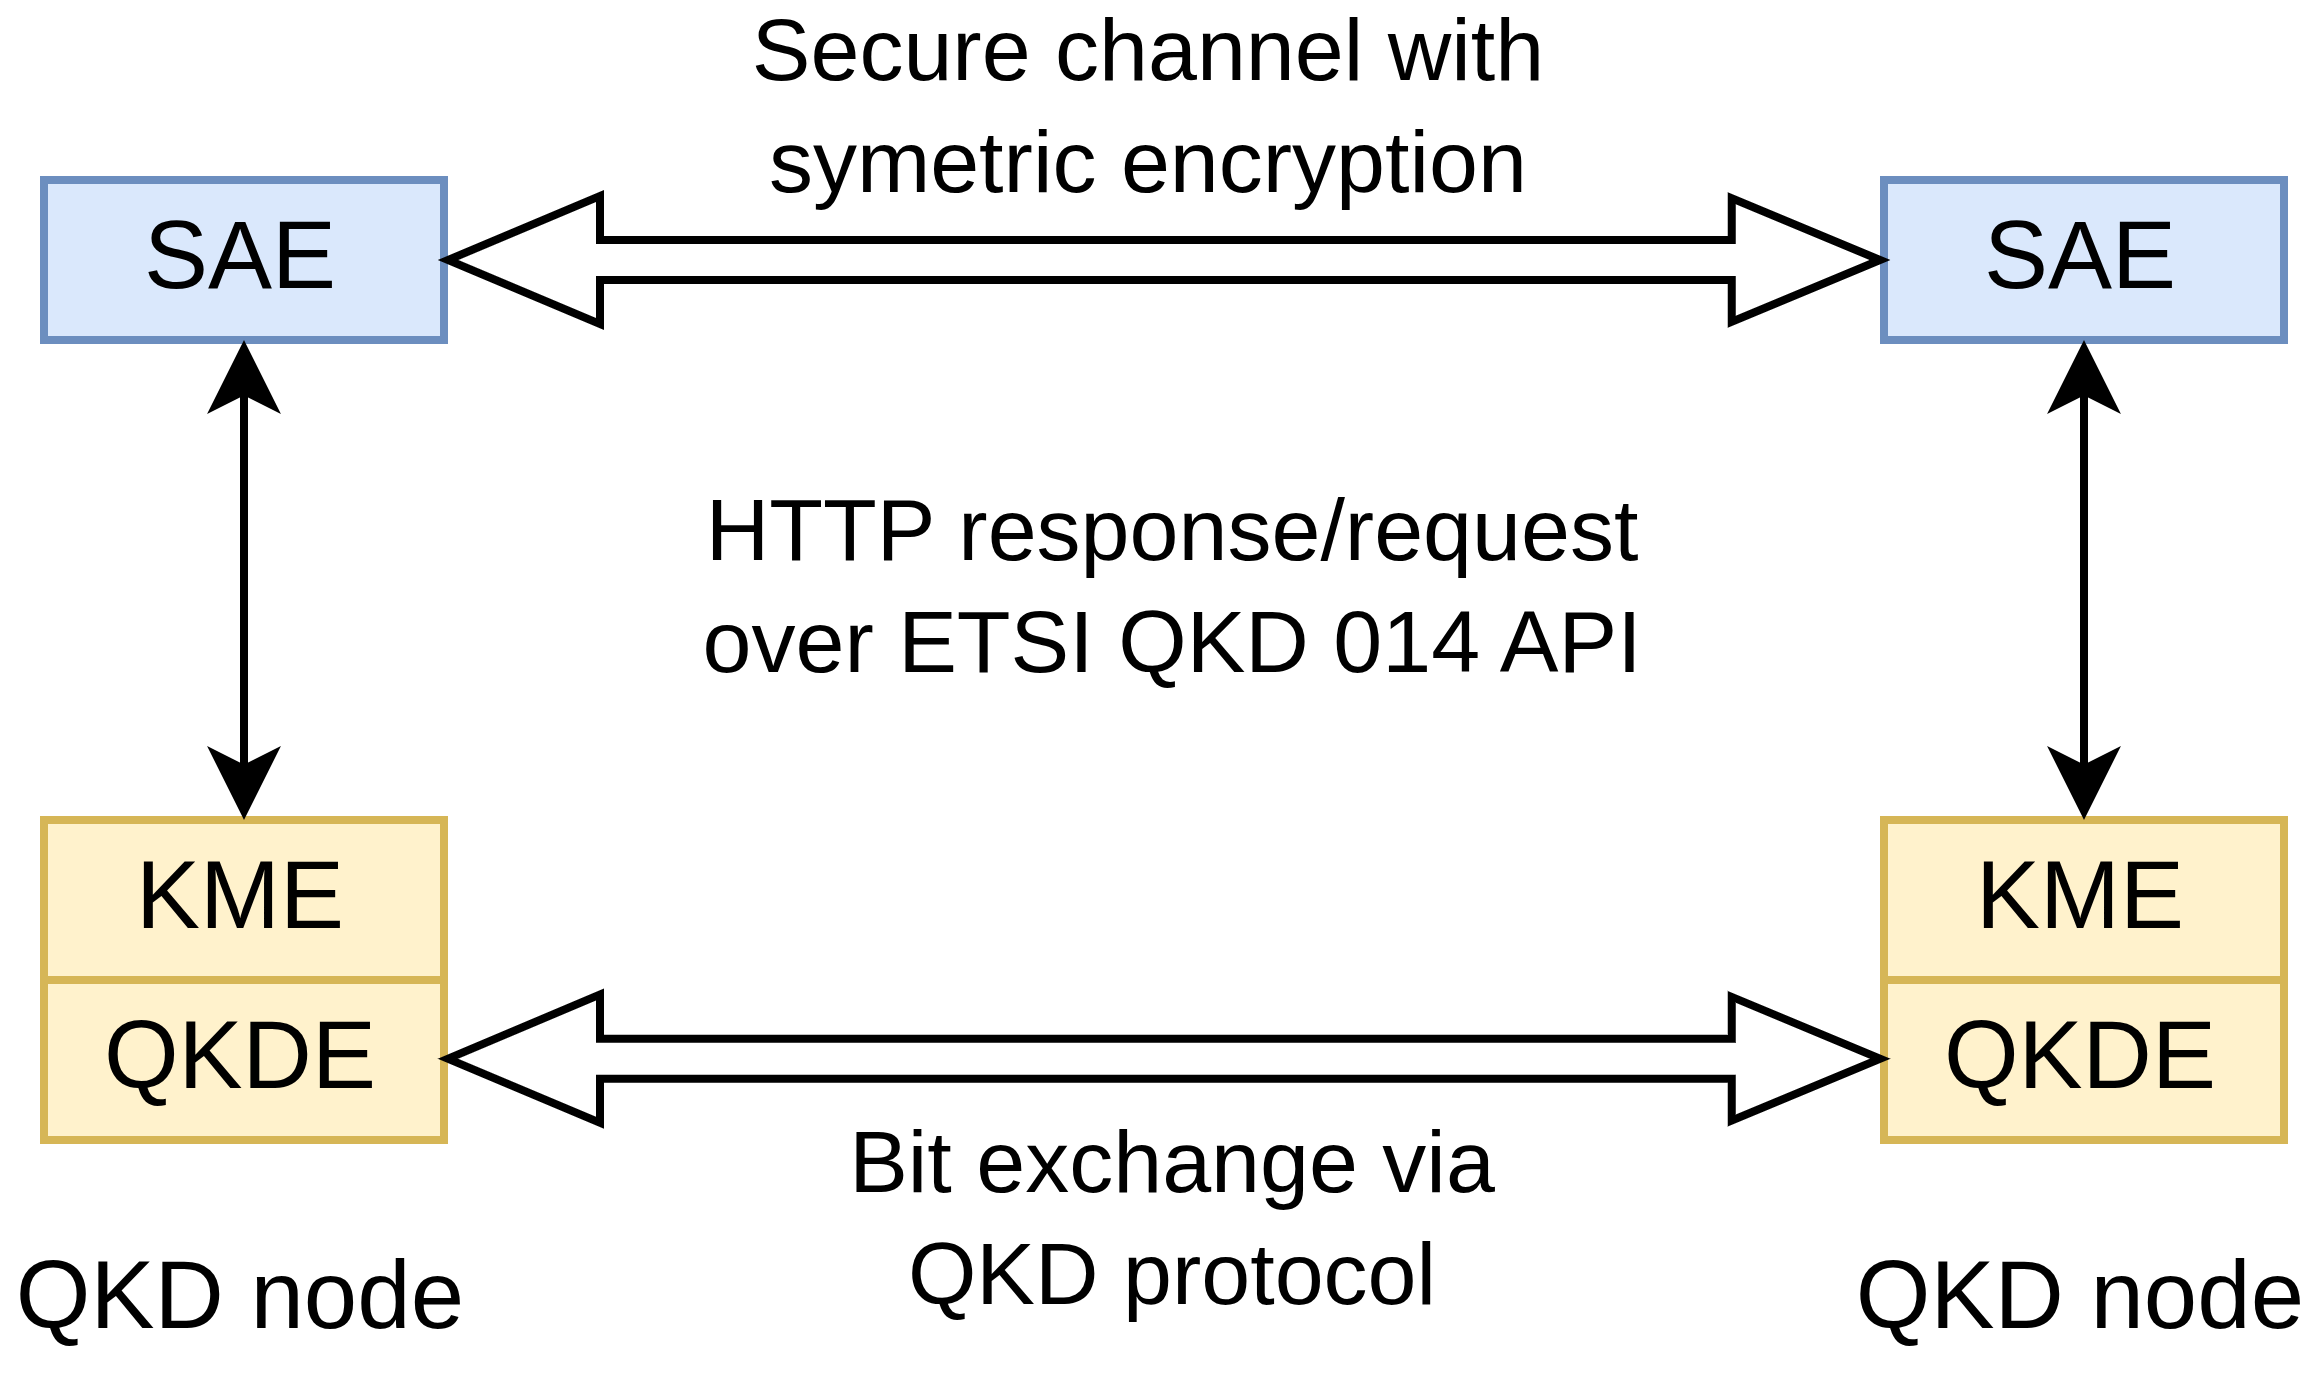
\includegraphics[width=7.7cm]{figures/qkd-link}
\caption{QKD link\label{fig:qkd_link}}
\end{figure}

Each QKD node has two parts: the QKD Entity (QKDE) and a Key Management Entity (KME). QKDEs are the devices that run QKD protocols, such as
BB84~\cite{bennett_quantum_2014} or BBM92~\cite{bennett_quantum_1992}, and end up with matching secret bits. KMEs, also known as quantum Key
Management Systems (KMS), are responsible for producing keys from these secret bits, securely storing those keys, applying key management policies and
delivering keys to authorized Secure Application Entities (SAE). According to QKD ETSI 014 API~\cite{noauthor_quantum_2019} standard SAEs are entities
that request one or more keys from a KME and represent applications running in cooperation with one or more other SAEs. After two peer SAEs receive
the corresponding keys, they can establish a secure channel with a symmetric scheme to protect the data exchange between them. In the context of
QTEE-V architecture secure relays represent these SAEs.

\subsection{Secure relay}

The main role of the relay is to forward keys along the QKD path. The relay is a process running inside a TEE on a remote device, at the QKD link
endpoints. On start up, each relay registers with the controller. During this process the relay generates the attestation report and sends it to the
controller. After the attestation report is verified and the relay has proven it is in a healthy and secure state, it waits for a message from its
neighbor relays. Upon receiving a message, the relay forwards it along the QKD path.

\subsection{Controller}

The role of the controller is relay registration and orchestration. The controller is process running on a remote server and it is assumed to be safe
(it is either running inside a TEE or on QKD owner's premises). As mentioned, on startup each relay registers with the controller. This process, which
will be described in detail in the subsequent sections, involves remote attestation, in which each relay must present a valid and fresh attestation
report to the controller. After verifying this report, the controller adds the relay to the system.

%%%%%%%%%%%%%%%%%%%%%
\section{QTEE-V Protocol}
In this section we describe the protocol that is used to achieve the secure key exchange. This protocol consists of only two message exchanges. The
first message exchange is relay registration with the controller which is done only once at relay startup. The second message exchange is relay
message forwarding which is performed each time a relay receives a message from one of its neighbors.

It is assumed that both the controller, the applications and the KMEs have access to a certificate authority (CA) which can sign and issue PQC certificates. These
certificates play a vital role in the protocol as will be explained in the following chapters. We deploy a dedicated private PKI rather than relying
on public certificate authorities. Public CAs do not currently issue the ML-DSA-65 certificates the system requires. A private root also limits trust
to a single pinned CA instead of the full set of public roots, and it lets the controller issue relay certificates only after successful enclave
attestation. In exchange, the deployment becomes responsible for protecting the CA key and for certificate lifecycle management.

\subsection{Registration}

Each relay has three parameters that are defined in its code at compile time: controllers IP address, root CA\textbf{ }certificate and an ID. The IP
address and the root CA certificate are needed for the TLS handshake with the controller. The certificate has to be hard coded since the system
doesn't use a public PKI. The relays ID is used during the registration process. Because these parameters are inside the relays code and the relay
code measurement is one part of the attestation report, the value of these parameters cannot be changed because any changes will be detected during
attestation verification stage of the registration process. The report is verified by comparing it with the report generated at compile time (before deployment).

As mentioned, at startup each relay registers with the controller. It first contacts the controller through the hard coded IP address and establishes
a PQC enabled TLS channel with the controller. During the handshake only the controller presents its PQC certificate since relays don't have a valid
certificate at this point. Controllers PQC certificate is issued beforehand by the CA. The relay verifies the controllers PQC certificate against the
root CA certificate. After establishing the TLS channel, the registration process takes place. It is divided into two phases. During the first phase
the relay performs the process of remote attestation and authenticates itself as is shown in Figure~\ref{fig:registration_phase1}.

\begin{figure}[H]
\centering
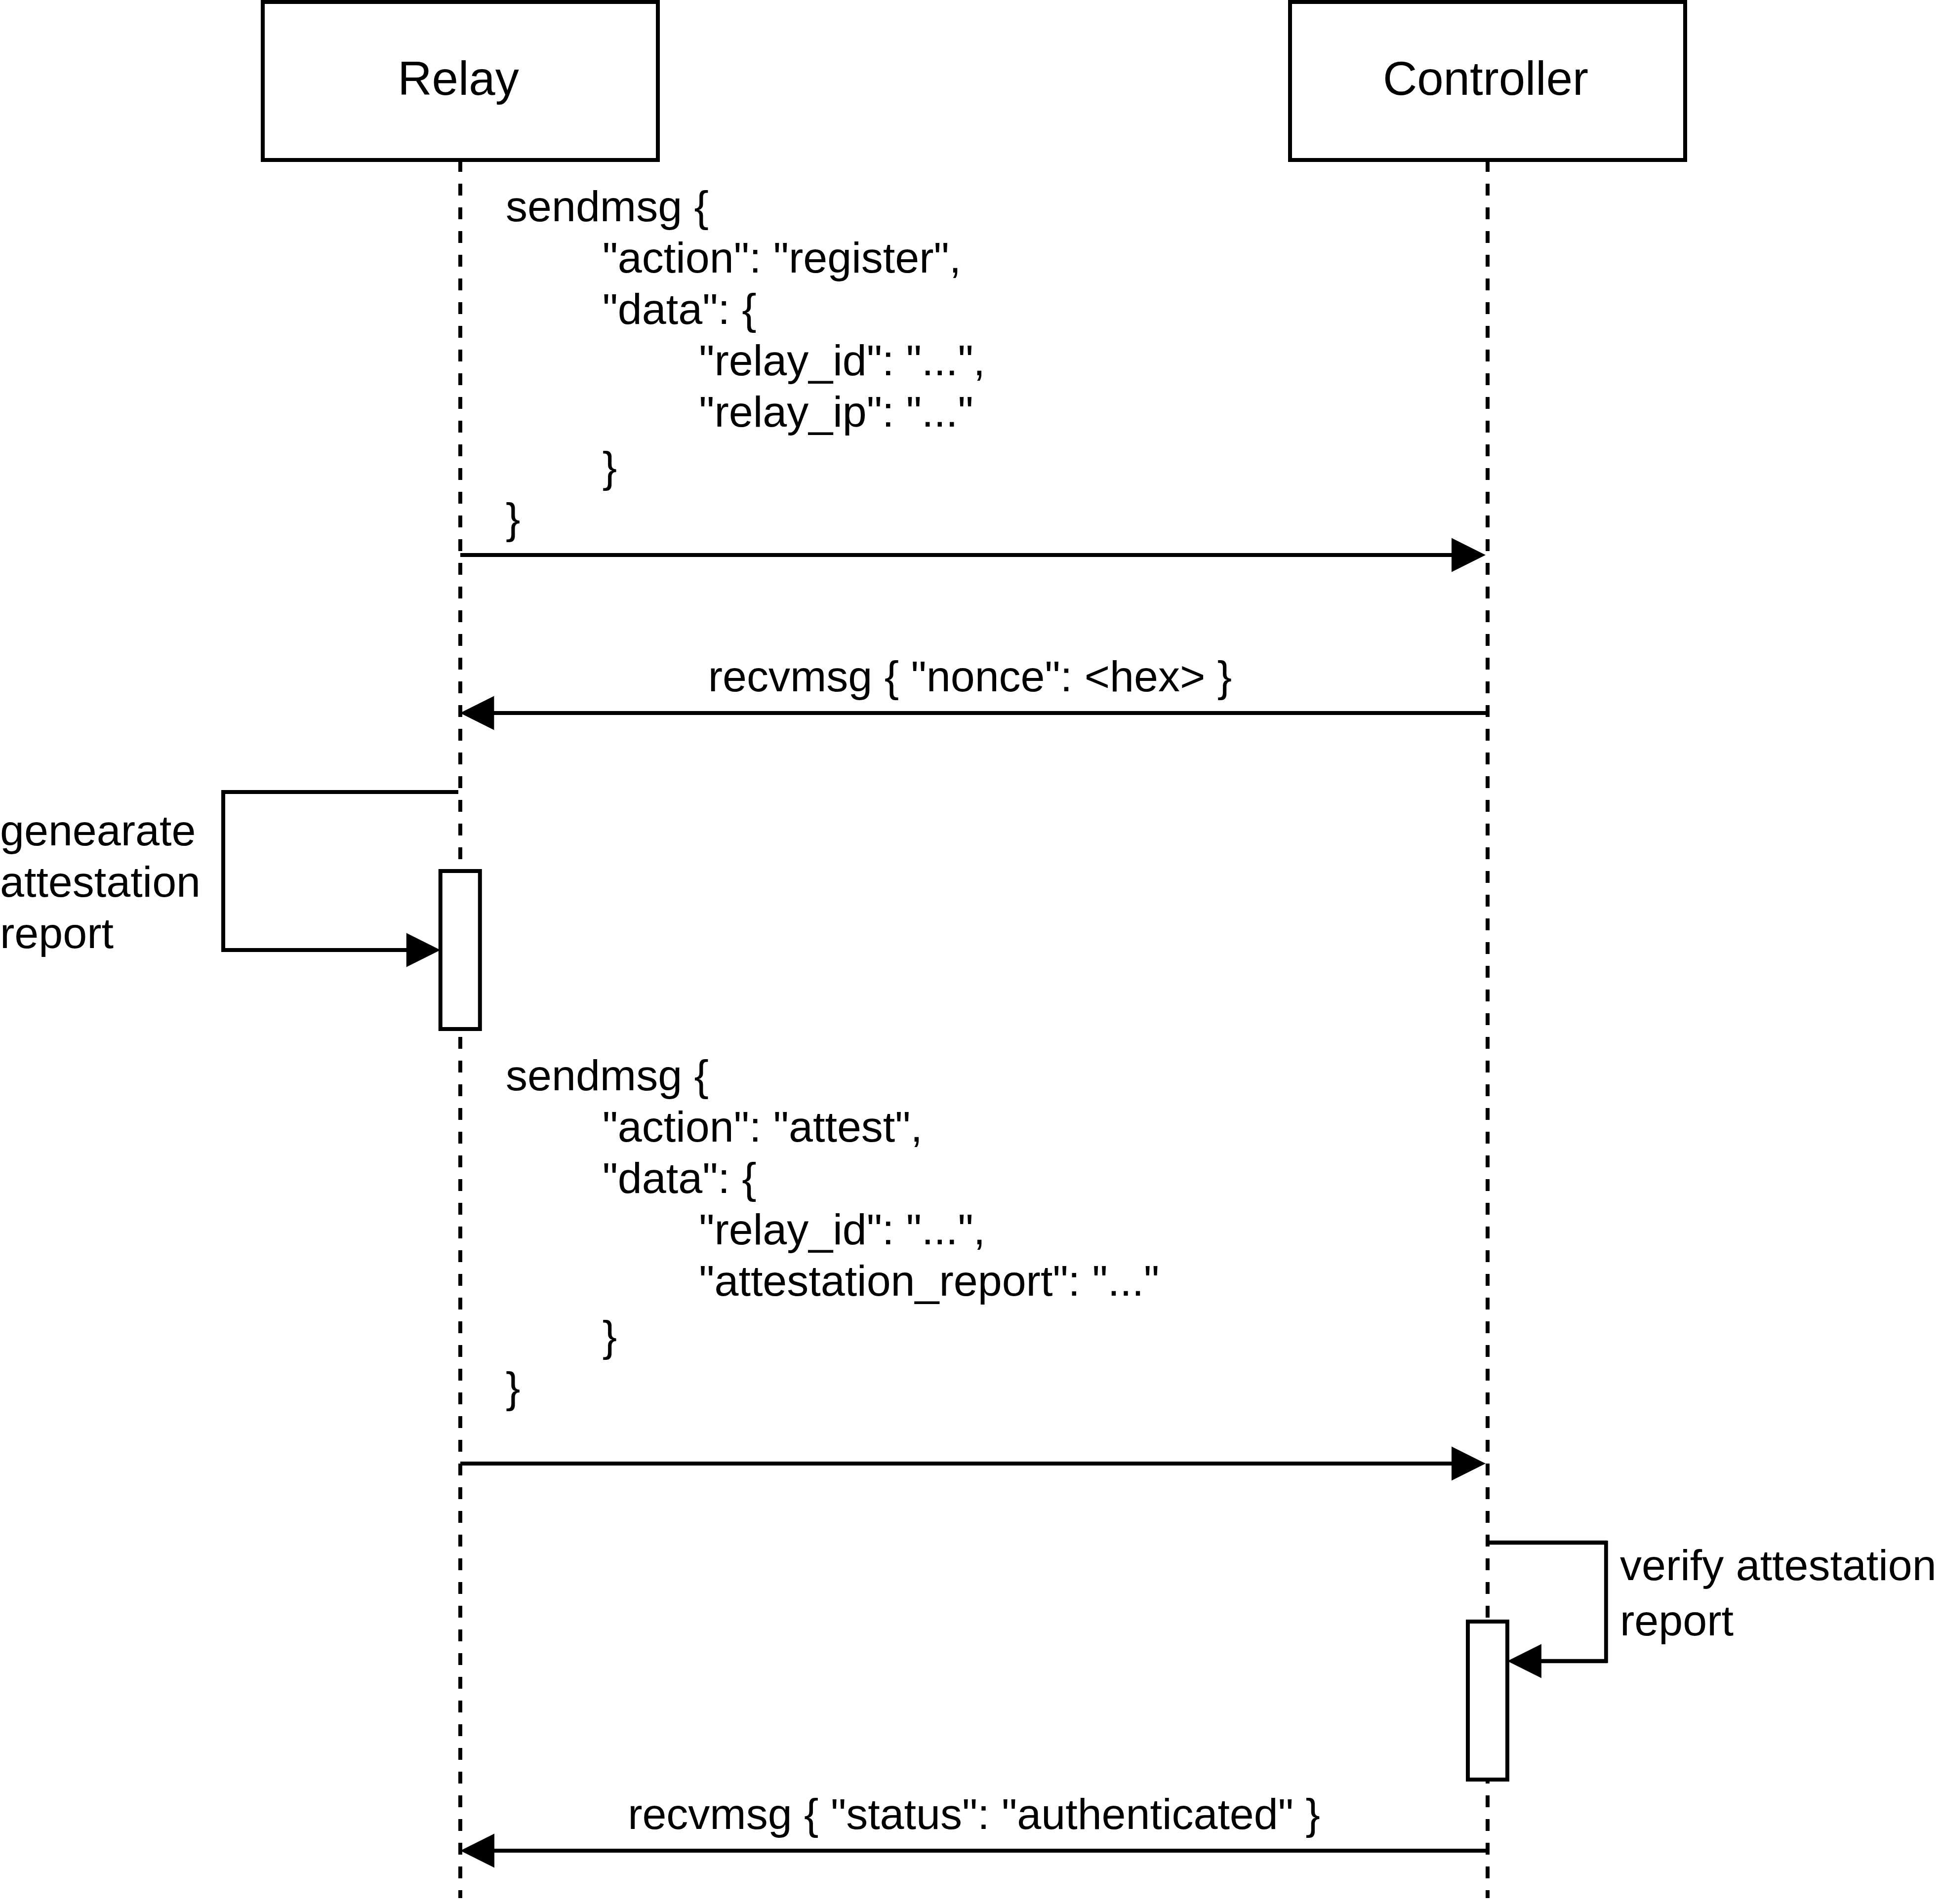
\includegraphics[width=13.0cm]{figures/relay-registration-phase1}
\caption{Relay registration, phase 1\label{fig:registration_phase1}}
\end{figure}

First, the relay sends a message to the controller indicating that it is ready to be authenticated. This message also includes relays ID and the
relays IP address. The relays ID and its IP address are included for two reasons. Firstly, because the registration process consists of multiple
steps, each relay needs to establish a session with the controller. This session is tied to the relays ID and the established TLS channel. Tying the
session to the TLS channel prevents the adversary from hijacking the session by misrepresenting himself as the relay (using its relay ID). Secondly, a
relays ID and IP address are used during message forwarding between relays. Therefore, they are needed for relay orchestration. The controller
responds with a nonce which is used to prove freshness of the attestation report.

The relay then generates the attestation report. The report includes hashes of relevant relay components i.e. the hash of SM, RT and relay binary. The
report also includes the provided nonce and the ID of the relay (it is compiled into the relay binary). The report is signed with the hardware
root of trust, i.e.,
\begin{equation}
\mathit{AR} = \mathit{Sign}\left(\mathit{SM}_{\mathit{hash}} \parallel \mathit{RT}_{\mathit{hash}} \parallel
\mathit{relay}_{\mathit{hash}} \parallel \mathit{nonce}, K_{\mathit{RoT}}\right).
\label{eq:relay_report}
\end{equation}
This approach guarantees freshness, because of the supplied nonce, and ties the attestation report to the relay ID because its compiled into the relay
binary. Next, the attestation report is sent to the controller for verification. If the verification by the controller is successful, the controller
notifies the relay that its ready to start the next phase which is shown in Figure~\ref{fig:registration_phase2}.

\begin{figure}[H]
\centering
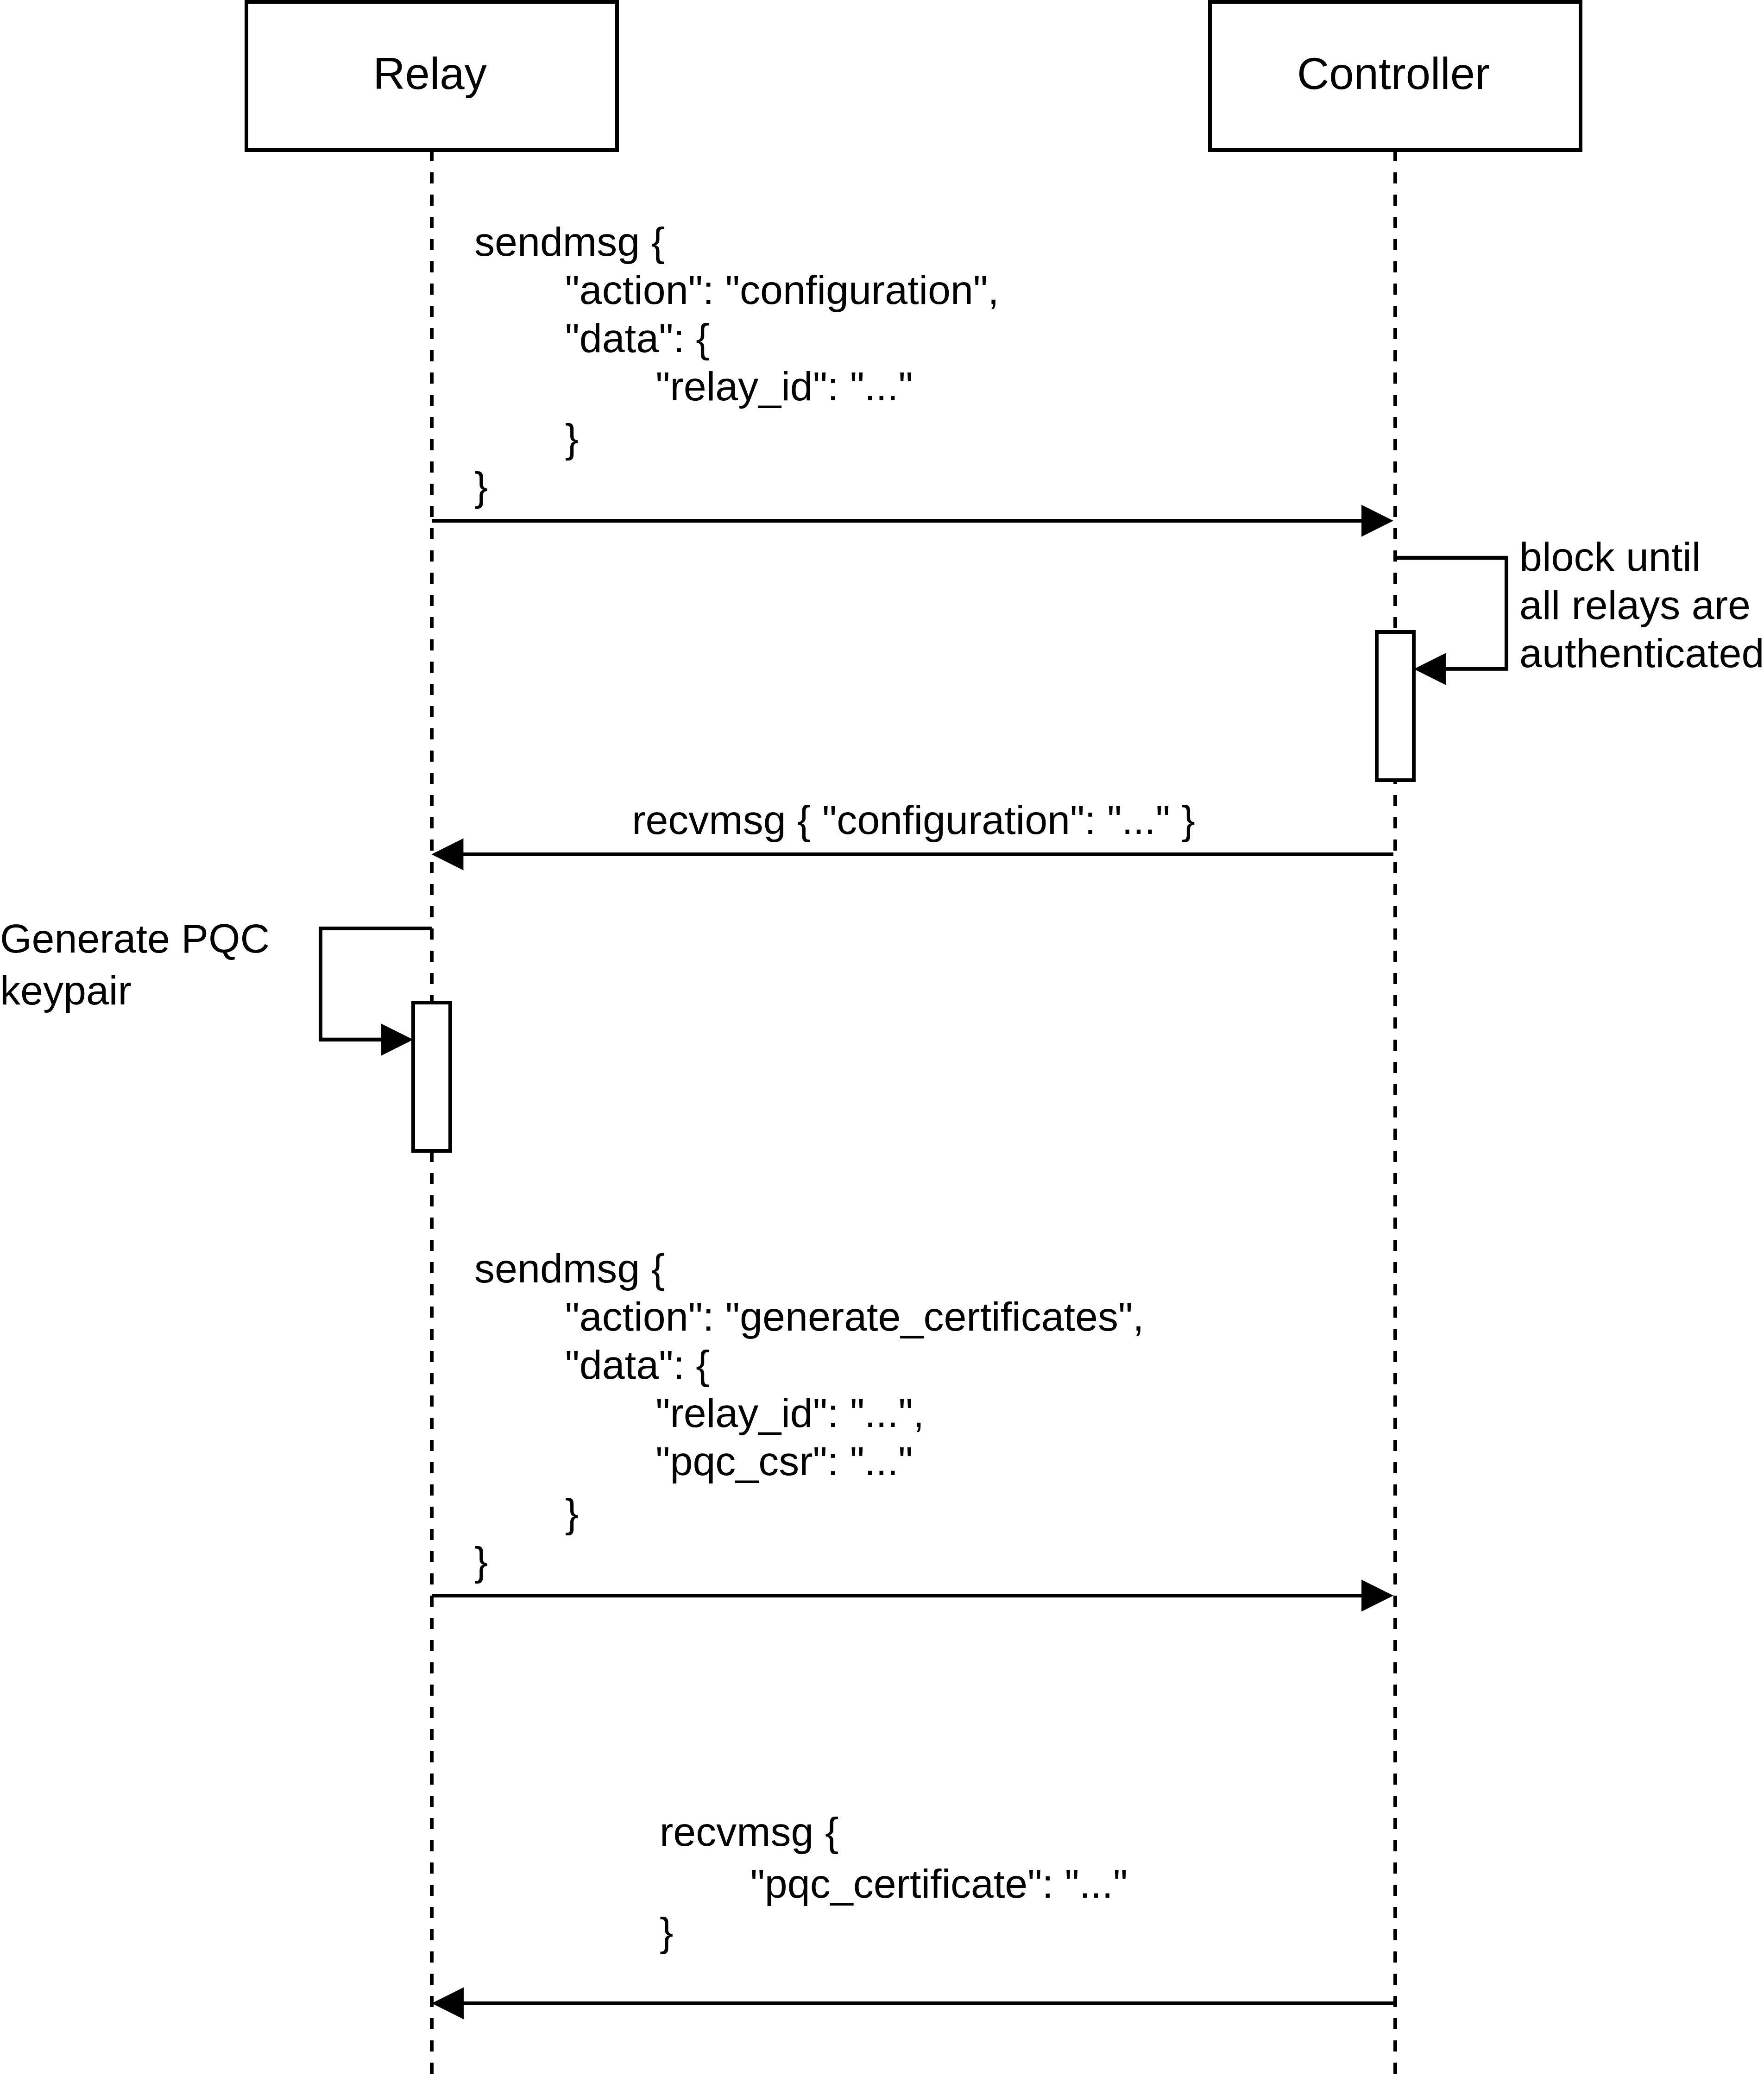
\includegraphics[width=11.0cm]{figures/relay-registration-phase2}
\caption{Relay registration, phase 2\label{fig:registration_phase2}}
\end{figure}

During the second phase, the relay requests the configuration data from the controller. Configuration data includes IP addresses and IDs of
neighboring relays, IP addresses of the neighboring KMEs and root CA certificate all of which are necessary for the message exchange with its
neighbors (relays or applications) which will be described later. After it receives the configuration, the relay generates a ML-DSA-65 (Dilithium 3)
key pair for a certificate it will use for communication with its neighboring relays and KMEs. The relay then sends the Certificate Signing Request
(CSR, based on the PKCS\#10 specification~\cite{nystrom_pkcs_2000}) to the controller. The controller forwards the request to its CA and returns the
generated ML-DSA-65 X.509 certificate to the relay.

After this step, the relay enters an idle state and waits for a connection from either neighbor (another relay or an application). Unlike the
registration channel, where only the controller presents a certificate, these connections use mutual TLS in which both endpoints authenticate with
X.509 certificates. For each handshake, an ephemeral ML-KEM-768 key pair is generated for key establishment. Authentication relies on ML-DSA-65. Each
endpoint signs the handshake transcript, which includes the ML-KEM-768 key share and ciphertext, with the private key corresponding to its
certificate. The peer verifies this signature using the public key from the certificate, after validating the certificate against the CA root. This
binds the established session key to the identity of the certificate holder.

It is important to note that the relays only receive a certificate if the process of remote attestation and relay authentication is successful. The
relay will present the issued certificate during the TLS handshake to prove that the attestation verification (registration) was successful and that
the relay is in a healthy and secure state. In addition, the Common Name (CN) field of each issued certificate is set to the corresponding relay ID.
The configuration data received from the controller specifies the IDs of the neighboring relays, and communication is restricted to these relays only.
The CN field of the certificates can therefore be used to enforce this communication restriction.

\subsection{Relay Message Forwarding}

Before the the main part of the protocol begins, all relays along the path must successfully go through registration and receive a PQC certificate issued
by CA. In addition, the applications at both ends of the path, that exchange keys via this system, also possess a PQC certificate issued by CA.
As with the relays, each application has its own unique ID which is used as the CN in the certificate and this ID is sent to the relays at the both ends of
the path during the registration process so that the relays can verify the application that is trying to contact them. During this part of the
protocol all communication is done inside a PQC enabled TLS channels and ML-KEM-768 is used for key exchange. In addition, every participant verifies
the certificate presented by its peer against root CA certificate.

The whole flow begins with the application (APP\textsubscript{0}) generating a key of arbitrary length (K\textsubscript{APP}). The application then
sends the key to the nearest relay over a PQC enabled channel. As with the application certificates, the IP of the nearest relay is issued beforehand
and the delivery method is outside the scope of the paper. The relay then forwards the key along the path. Control flow for exchanging messages
between relays is depicted in Figure~\ref{fig:message_forwarding}.

\begin{figure}[H]
\centering
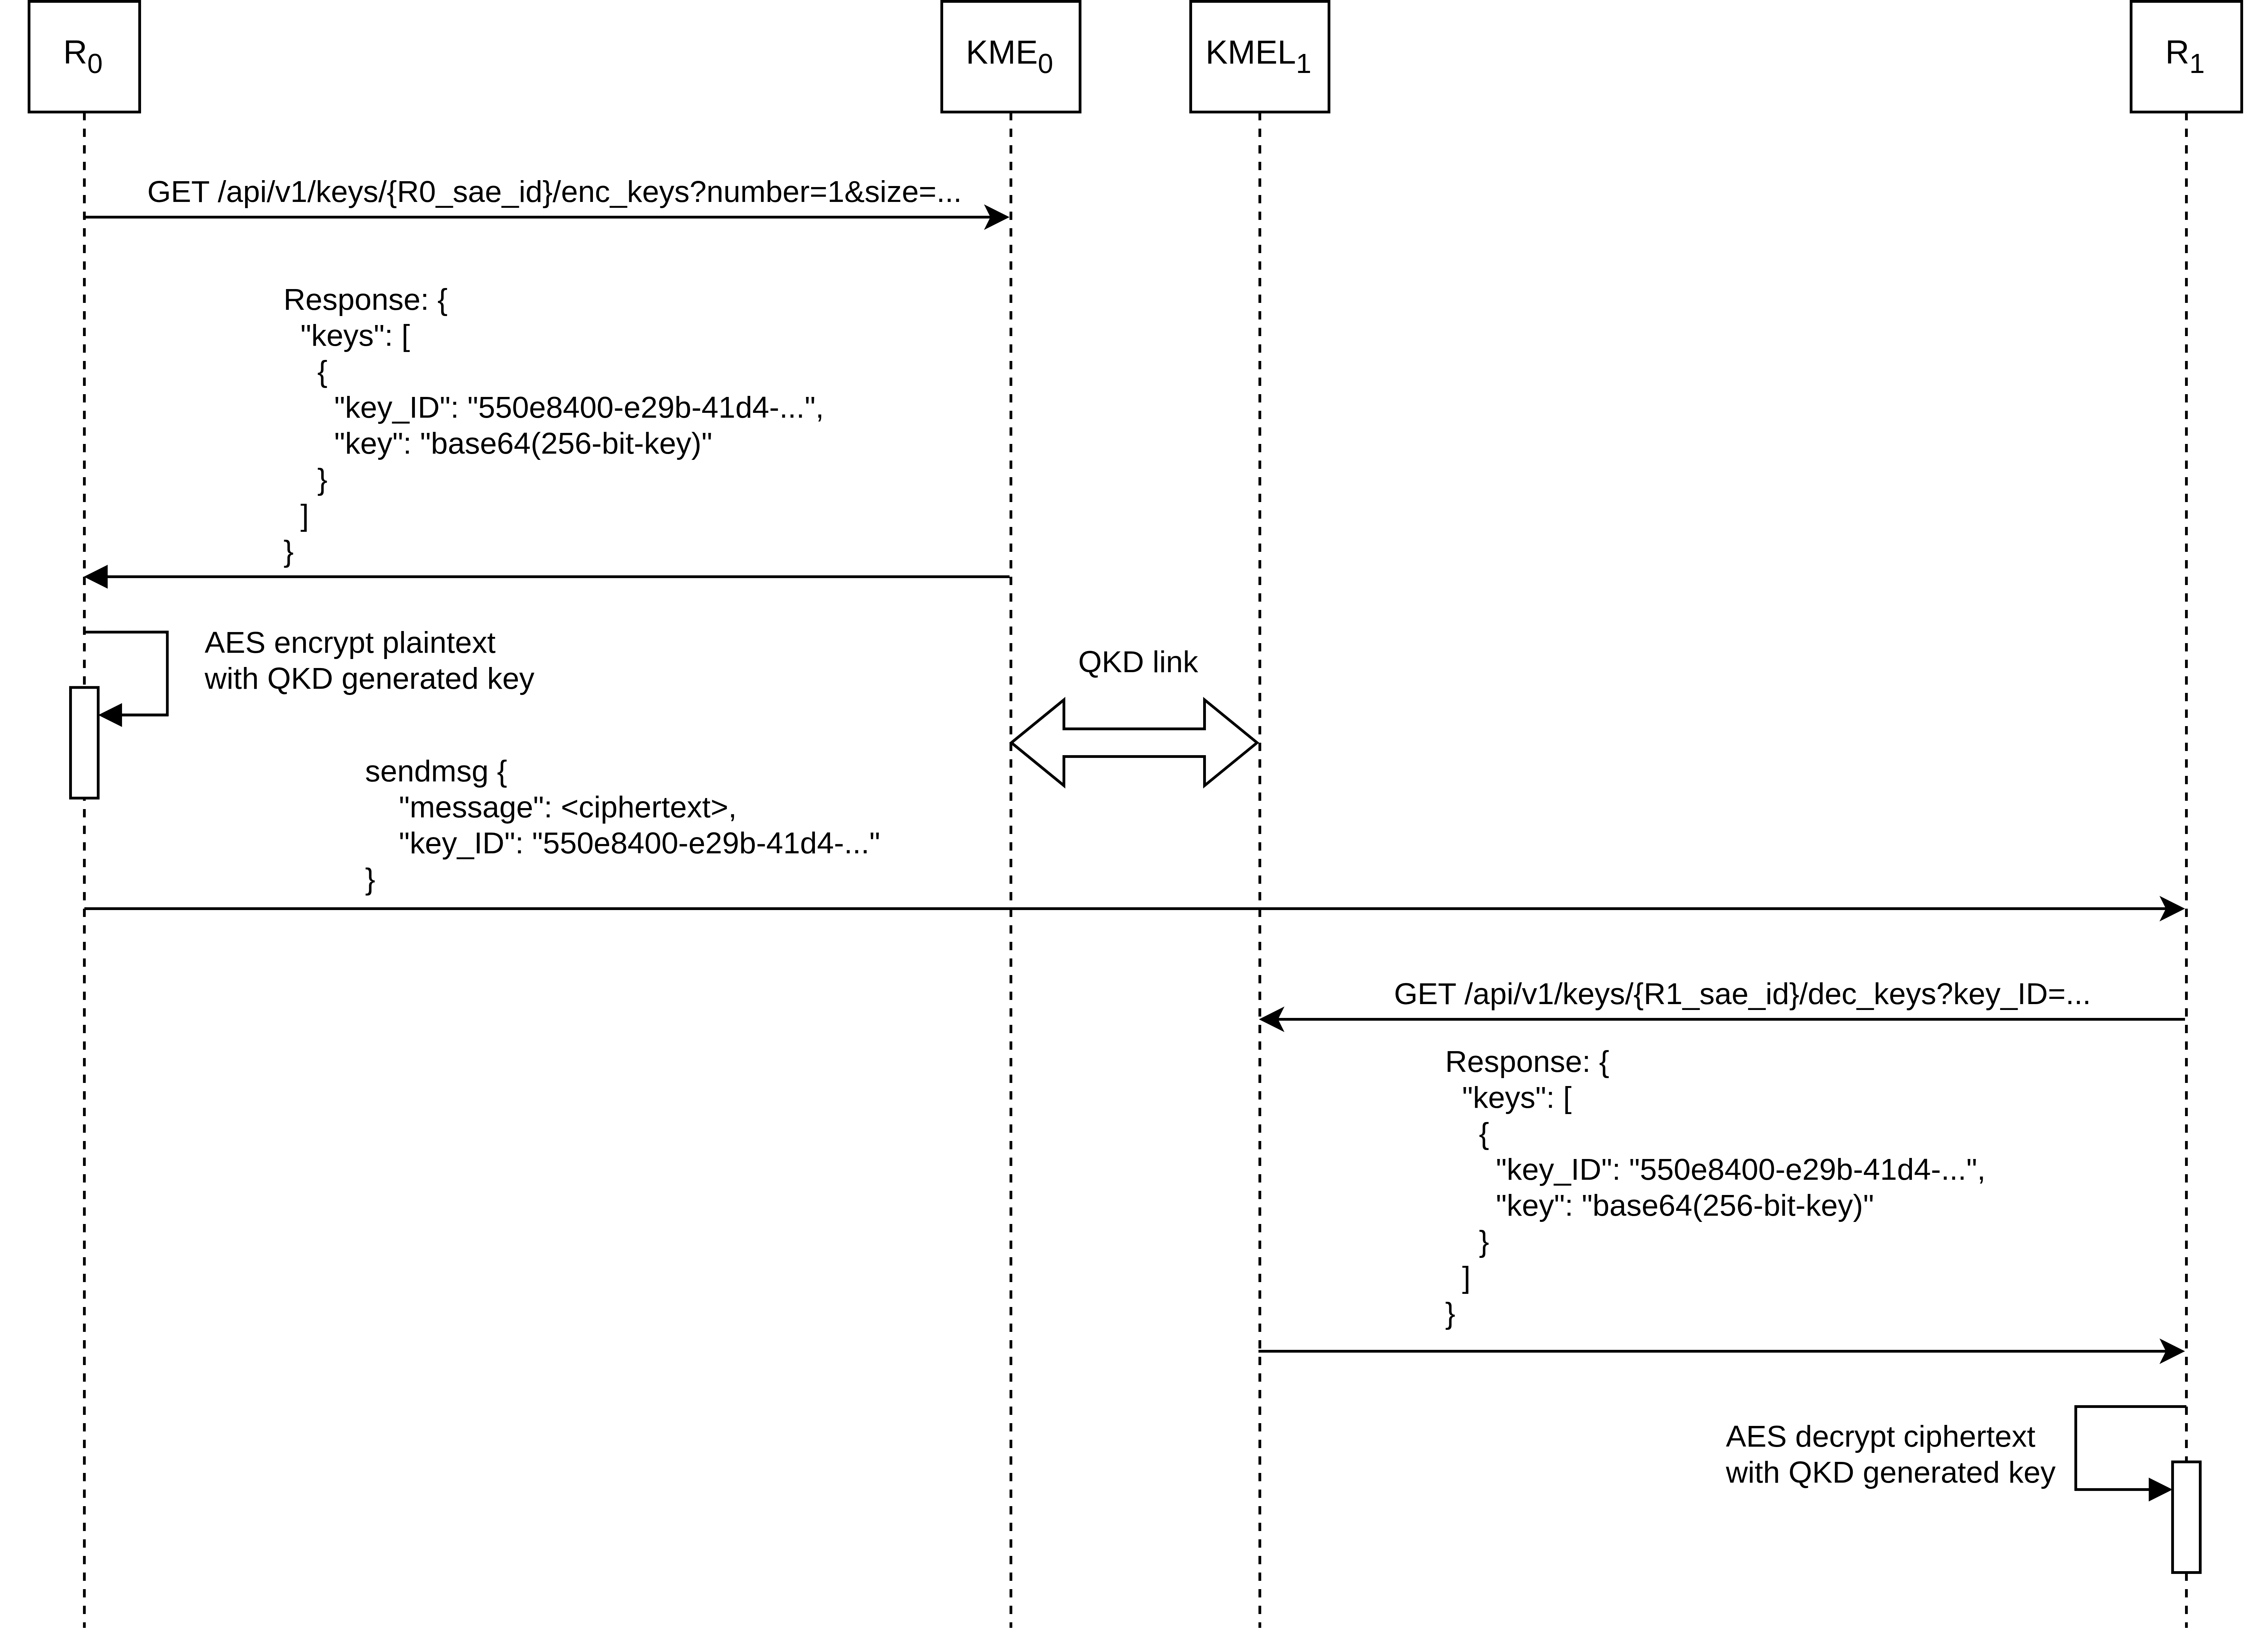
\includegraphics[width=\linewidth]{figures/message_forwarding}
\caption{Relay Message Forwarding\label{fig:message_forwarding}}
\end{figure}

When a relay R\textsubscript{0} wants to forward K\textsubscript{APP} key to relay R\textsubscript{1}, it first needs to encrypt K\textsubscript{APP}
with a key (K\textsubscript{QKD}) generated by the underlying QKD link. After establishing a PQC enabled TLS channel with the KME of first node of a
QKD link (KME\textsubscript{0}), the relay R\textsubscript{0 }asks KME\textsubscript{0} to generate a key using requests described in QKD ETSI 014 API
standard~\cite{noauthor_quantum_2019}. The relay requests a key via GET request which has three parameters: SAE ID of the recipient relay (the ID of
relay R\textsubscript{1}), number of keys and size of the keys. The response from the QKD node is a list of keys and their IDs (in this case the list
has only K\textsubscript{QKD }and the ID with which it can be retrieved). Next, the R\textsubscript{0 }relay encrypts the K\textsubscript{APP} using
the AES algorithm and the K\textsubscript{QKD} key. After the encryption, the R\textsubscript{0} relay establishes a PQC enabled TLS channel with the
R\textsubscript{1} relay. After the channel is established, the R\textsubscript{0} relay sends the encrypted payload (encrypted K\textsubscript{APP})
and the ID of the K\textsubscript{QKD}. After receiving the message, the R\textsubscript{1} establishes a PQC enabled channel with the KME of second
node of the QKD link (KME\textsubscript{1}). After the channel is established, R\textsubscript{1} retrieves the K\textsubscript{QKD }key via GET
request which has two parameters: SAE ID of the R\textsubscript{0} relay in order to know the origin of the generated key and ID of the
K\textsubscript{QKD} key. After receiving the K\textsubscript{QKD }key, the R\textsubscript{1} relay decrypts the payload using AES algorithm and the
K\textsubscript{QKD }key\textsubscript{ }and retrieves K\textsubscript{APP }in plain text. This process is repeated for each hop along the path.
However, if the recipient or the sender is the application at either end of the path there is no encryption via AES. These exchanges are done inside a
PQC enabled TLS channel.

%%%%%%%%%%%%%%%%%%%%%
\section{QTEE-V Implementation}

In this section we will describe the implementation details. This sections also includes the description of the external components used to implement
this system. All source files with the instructions on how to start and test the system are available at~\cite{dukic_qtee-v_2026}.

\subsection{QTEE-V communication}

All communication is implemented using WolfSSL~\cite{wolfssl_inc_wolfssl_nodate} since its designed to be an embedded, lightweight and portable
C-language-based TLS library. WolfSSL supports ML-DSA~\cite{national_institute_of_standards_and_technology_us_module-lattice-based_2024-1}, which is
used by the controller for certificate signature, and ML-KEM~\cite{national_institute_of_standards_and_technology_us_module-lattice-based_2024}, which
is used during the key exchange.

The library is compiled for the RISC-V architecture and it is statically linked to the relay application running inside a TEE. Furthermore, it is
configured to use the random number generator provided by the Keystone SM in order to avoid using the random number generator provided by the Rich
Execution Environment (REE) which is considered untrusted. As we will describe in the next chapter, a number of syscalls are proxied to the REE and
with this approach we are sure that the keys generated using WolfSSL library aren't compromised.

\subsection{RISC-V enclave}

The relay is running inside RISC-V Keystone secure enclave. The Keystone platform is an open source project that leverages RISC-V PMP in order to
enable developers to create secure enclaves. Figure~\ref{fig:keystone_architecture} gives an overview of the RISC-V Keystone architecture.

\begin{figure}[H]
\centering
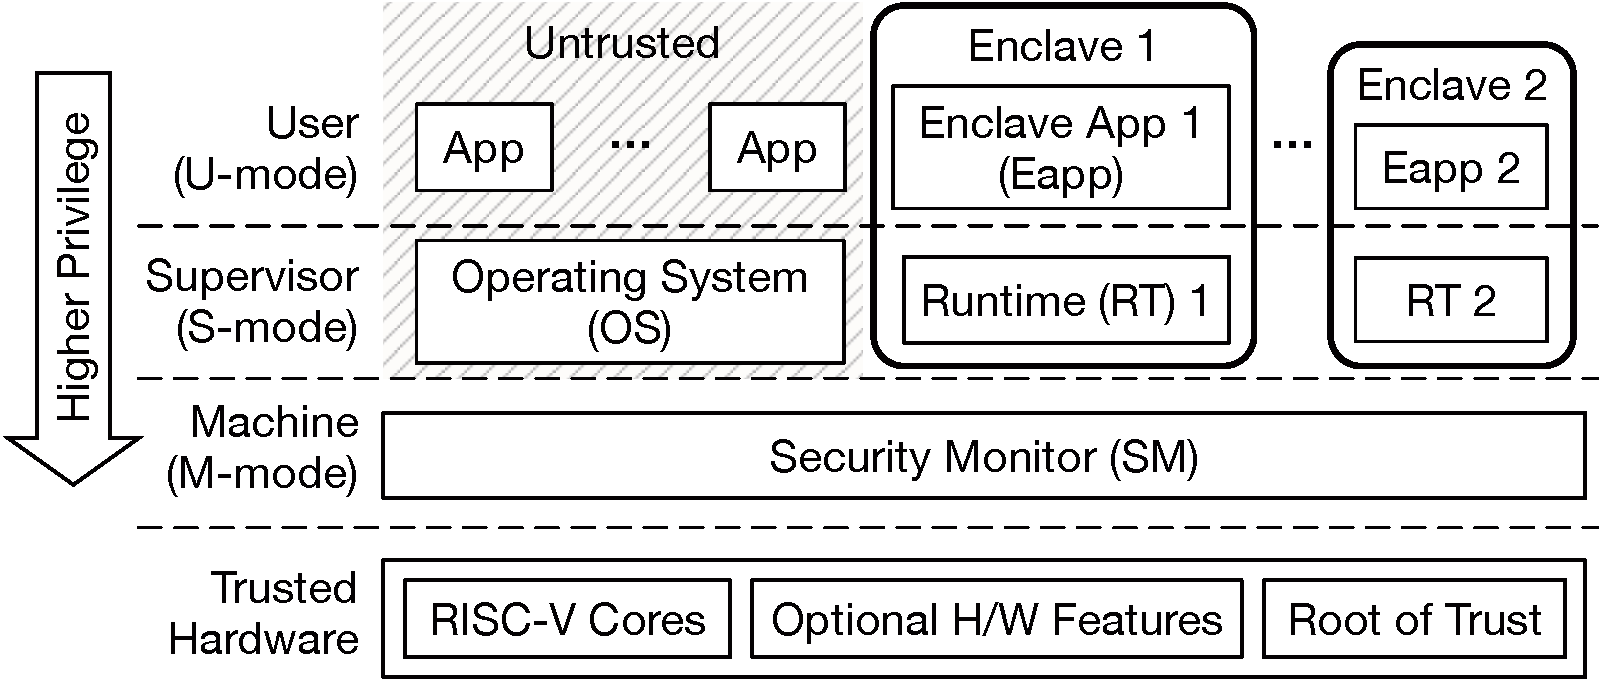
\includegraphics[width=\linewidth]{figures/keystone_architecture}
\caption{RISC-V Keystone architecture~\cite{lee_keystone_2019}\label{fig:keystone_architecture}}
\end{figure}

The main components of the Keystone platform are the Secure Monitor (SM), the Runtime (RT) and the Secure Enclave (E\textsubscript{APP}). Secure
Monitor executes in M-mode which has the highest privileges. M-mode is the only mode that has access configuration registers that enable/disable
memory isolation provided by the PMP unit. In addition, Security Monitor is also responsible for enclave lifecycle management, switching between the
untrusted Rich Execution Environment (REE) and Secure Enclaves and other enclave services, including enclave attestation. The attestation report is
generated by hashing the SM code, the RT code and the E\textsubscript{APP} code. In addition, it includes a provided nonce which ensures freshness and
the whole payload is then signed with the HW root of trust, i.e.,
\begin{equation}
\mathit{AR} = \mathit{sign}\left(\mathit{EAPP}_{\mathit{hash}} \parallel \mathit{RT}_{\mathit{hash}} \parallel \mathit{SM}_{\mathit{hash}} \parallel
\mathit{nonce},\; K_{\mathit{RoT}}\right).
\label{eq:keystone_report}
\end{equation}
HW root-of-trust can be implemented in various ways as is explained in the Keystone framework paper~\cite{lee_keystone_2019}, but the authors decided
to keep the implementation adopted in the paper (it is implemented as a variable in the code base).

RT implements a limited range of system calls. System calls that are not implemented in the RT are forwarded from the E\textsubscript{APP} to the host
application by re-using the edge call interface. The user host application then invokes the syscall on an untrusted OS on behalf of the
E\textsubscript{APP}, collects the return values, and returns them to the E\textsubscript{APP}. There are two runtimes available out of the box: Eyrie
and seL4~\cite{klein_sel4_2009}. The authors opted for the former because it is already a part of the Keystone framework code base. For certain
operations (e.g. generating the attestation report), RT communicates with the SM via OpenSBI~\cite{risc-v_international_risc-v_2022}.

The relay itself is implemented as a normal C process. Since the Eyrie RT follows the Linux system call naming convention, no changes need to be made
to C program itself other than to include Keystone headers that provide enclave specific functionalities like generating the attestation report.

\subsection{QKD simulator}

QKD systems are still in the early stages of development and there aren't many devices available for developing and testing. Therefore, for the
purposes of this paper we used a simulator called Next door key simulator~\cite{garkaklis_next_2023}. One drawback with this simulator is that it
doesn't support PQC. Therefore, the authors added PQC support which is implemented as a proxy service running in the same container as the simulator.
This service handles all PQC enabled communication and forwards the original requests as non-PQC requests to the original simulator. In addition, the
controllers CA\textsubscript{RELAY} root certificate is added to the container in order to enable relay certificate verification. Since the
certificate is issued to relays only after successful attestation, if the certificate verification is successful, the simulator can be sure that its
communicating with relay in a healthy and secure state.

\subsection{Putting it all together}

As we mentioned at the begging of this chapter, the whole code base for the QTEE-V system is available at~\cite{dukic_qtee-v_2026}. This repository
includes the Keystone framework repository and the Next door key simulator repository, both with changes necessary for the QTEE-V system to work. It
also includes detailed instructions on how to test the whole system. The testbed is the same as in Figure~\ref{fig:architecture} and consists of the
following components:

\begin{itemize}
\item 4 docker containers from the modified Next door key simulator that represent two QKD links
\item 2 relay processes running as python scripts which represent relays R0 and R2
\item 1 relay process running inside RISC-V Keystone TEE which represents relay R1
\item 1 controller running as a python script
\item 2 python applications on either end of the path that exchange keys via the system
\end{itemize}

There is python script inside the repository that demonstrates the proposed architecture and protocol and produces logs covering the following
scenarios:

\begin{itemize}
\item \textbf{Scenario 1}: The whole protocol is executed without errors
\item \textbf{Scenario 2}: Peer certificate CN absent from whitelist and the connection is rejected by the relay
\item \textbf{Scenario 3}: Certificate is signed by a different CA and relay rejects he connection during the handshake
\item \textbf{Scenario 4}: A relay makes a key request to the KME without a valid certificate and the connection is refused
\item \textbf{Scenario 5}: The attacker replays the attestation report from an earlier session replayed which results in the controller
\item \textbf{Scenario 6}: The enclave image is modified which results in measurement mismatch during registration
\end{itemize}

In addition to demonstrating that the architecture and protocol are working and safe, these scenarios also demonstrate the security properties which
are discussed in the following chapter. For brevity, only parts of the logs from the first scenario are presented. These parts cover the the
attestation process and the message exchange and are presented in Listings~\ref{lst:attestation_logs} and~\ref{lst:forwarding_logs}.

\begin{listing}[H]
\caption{Attestation logs.\label{lst:attestation_logs}}
\rule{\columnwidth}{1pt}
\begin{lstlisting}
00:00:01.436 [R1·enclave] [DEBUG] Using hardcoded CA cert (5436 bytes DER)
00:00:01.436 [R1·enclave] [DEBUG] Connecting to controller TLS on 192.168.100.2:8001...
00:00:01.440 [CTRL      ] [TLS] New connection from ('127.0.0.1', 43978)
00:00:01.554 [CTRL      ] [TLS] server handshake group: ML_KEM_768
00:00:01.554 [CTRL      ] [TLS] Handshake complete with ('127.0.0.1', 43978)
00:00:01.563 [R1·enclave] [DEBUG] WolfSSL TLS connected to controller, server cert verified
00:00:01.563 [R1·enclave] [DEBUG] Sending register...
00:00:01.564 [CTRL      ] [R1] Register
00:00:01.565 [CTRL      ] [R1] Nonce: a3deaad9156b561e49d604a...
00:00:01.568 [R1·enclave] [DEBUG] Received 00=a3deaad9156b561e49d604a...
00:00:01.573 [R1·enclave] [DEBUG] Sending attest...
00:00:01.592 [CTRL      ] [R1] Keystone report verified: enclave=... sm=...
00:00:01.592 [CTRL      ] [R1] Authenticated (platform=riscv)
00:00:01.592 [CTRL      ] [R1] Registered (index 1)
\end{lstlisting}
\rule{\columnwidth}{1pt}
\end{listing}

\begin{listing}[H]
\caption{Message exchange logs.\label{lst:forwarding_logs}}
\rule{\columnwidth}{1pt}
\begin{lstlisting}
00:00:01.331 [R0        ] Forwarding ciphertext
00:00:01.334 [R1·enclave] Connection from 0.0.0.0
00:00:01.406 [R0        ] [TLS] client handshake group: ML_KEM_768
00:00:01.408 [R0        ] PQC mTLS connected to R1 at 127.0.0.1:9001
00:00:01.473 [R1·enclave] PQC TLS from R0
00:00:01.476 [R0        ] Received ack: RECEIVED
00:00:01.476 [R0        ] Message forwarded successfully
00:00:01.477 [R0        ] PQC mTLS listener on 0.0.0.0:9000
00:00:01.480 [R1·enclave] From R0
00:00:01.481 [R1·enclave] Getting decryption key from KME 192.168.100.2:8011 key_ID=...
00:00:01.646 [R1·enclave] Decrypting with QKD key key_ID=...
00:00:01.650 [R1·enclave] Plaintext: QTEE-V demo payload: application key ... for APP_R
00:00:01.651 [R1·enclave] Getting encryption key from KME 192.168.100.2:8012...
00:00:01.816 [R1·enclave] Encrypting with QKD key key_ID=...
00:00:01.818 [R1·enclave] Forwarding ciphertext
\end{lstlisting}
\rule{\columnwidth}{1pt}
\end{listing}

%%%%%%%%%%%%%%%%%%%%%
\section{Threat model and security}\label{sec:threat_model}

QTEE-V architecture and protocol protect the application key transported along the path, the QKD-derived hop keys, the relay credentials issued by
the controller, and the configuration that defines each relay's position in the system. From these we derive five security objectives:

\begin{itemize}
\item \textbf{G1 (Payload confidentiality)}---K\textsubscript{APP} must remain secret at every point of its journey, including while it is being
processed inside a relay, and including against software running on the relay device outside the enclave;
\item \textbf{G2 (Hop key confidentiality)}---No hop key may become known to any party other than the two relays sharing that QKD link;
\item \textbf{G3 (Attested admission)}---Only a relay that is genuinely executing the expected enclave image on genuine hardware may obtain a
certificate and join the system;
\item \textbf{G4 (Topology binding)}---A relay may accept a payload from, and forward a payload to, only those neighbors assigned to it by the
controller;
\item \textbf{G5 (Long-term confidentiality)}---All classical channels must resist an adversary who records traffic today and possesses a
cryptographically relevant quantum computer later.
\end{itemize}

\subsection{Trust assumptions}

The authors trust the RISC-V processor package, its PMP unit and its hardware root of trust. We assume the PMP unit provides isolation correctly and
that no application from REE can access TEE memory. We also assume that the integrity of the device is such that its memory cannot be physically
accessed from outside. This assumption is necessary since the PMP provides only isolation and no encryption. Finally, the cryptographic libraries and
randomness sources are assumed to provide their specified security properties. The correctness of the Keystone framework and its components (SM, RT
and E\textsubscript{APP}) can be verified through the attestation report.

The authors also trust the controller and QKD nodes and links. The controller runs inside a TEE in the cloud or on premise and that its in a secure
and safe state. The QKD layer is assumed to provide information-theoretically secure symmetric key material to the two KMEs associated with a link.
The KMEs are further assumed to securely store the generated link keys and release them only to SAEs that present a valid certificate.

\subsection{Adversary}\label{sec:adversary}

We consider an adversary with the following capabilities:

\begin{itemize}
\item The adversary has network control and can observe, drop, reorders, replays, modifies and injects messages on every classical link, spoofs
addresses and identities;
\item The adversary has quantum capability which means that he can record traffic for later decryption;
\item The adversary can compromise the REE of a relay device and get full privileges in the rich execution environment. However, he cannot
read or write enclave memory (enforced by PMP) and cannot have a modified image attested;
\item The adversary can learn a relay identifier and attempt to register a device or binary of its own, or replays a captured attestation
report;
\item The adversary can reach a deployed relay device, disconnect it, power-cycle it, replace its storage medium and reflash the untrusted software
image but he cannot mount an invasive attack on a running CPU;
\end{itemize}

It is important to note that the adversary cannot deploy a stolen relay binary on any other device because the HW root-of-trust signing key is not 
public. Therefore the adversary cannot generate a valid attestation report. In addition, the adversary cannot compromise the 
controller or the QKD layer.

\subsection{Limitations}

As with every system, there are certain limitations that are not addressed in this paper. The main limitation is \textbf{memory confidentiality}. PMP
isolates enclave memory from other software but does not encrypt it, and memory encryption is not currently a ratified RISC-V extension. An adversary
able to probe the memory bus or perform a cold-boot recovery on a running relay can obtain the payload key.

\textbf{The second most impactful limitation come from the fact that the attestation is a one-time admission check.} A relay proves its state at
registration and is then trusted for the lifetime of its certificate. A compromise that occurs after admission is not detected by the controller.

\textbf{The final limitation is the implicit trust in the controller and the QKD layer.} All admission decisions depend on one controller and one CA
key. Compromise of that key allows an adversary to certify arbitrary nodes as relays. In addition, the proposed architecture and protocol do not
protect against a compromised KME, a compromised QKD entity, or attacks on the physical quantum channel, and it inherits the trust assumptions of ETSI
GS QKD 014~\cite{noauthor_quantum_2020} key delivery.

%%%%%%%%%%%%%%%%%%%%%
\section{Verification}

We evaluate the modeled security of the QTEE-V system using ProVerif~\cite{blanchet_modeling_2016} against the active network adversary defined in
Section~\ref{sec:threat_model}. The model includes a controller, three relay identities R0--R2 and two application identities APP\_L and APP\_R. We
formalize the cryptographic assumptions and security requirements, then report security and reachability results for admission and bidirectional
forwarding.

\subsection{Formalization of the QTEE-V protocol}

All traffic uses a public channel net controlled by an active Dolev--Yao adversary as described in Section~\ref{sec:adversary}. The Relay CA root
certificate and hardware attestation keys are not compromised. Verification keys and expected reference measurements are public. Digital signatures
guarantee authenticity and integrity, but do not hide the signed messages.

The relays hardware signing key is represented with private function \texttt{hw\_sk(relay\_id)}. This key is used for signing the attestation report
during the registration process. Each report is represented with a tuple \texttt{(relay\_id, nonce, measurement)}, where \texttt{nonce} is the
challenge received during registration to prevent replay attacks. Controller accepts only the expected measurement and its own fresh challenge signed
by \texttt{hw\_sk(relay\_id)}. The constructor \texttt{cert\_make(relay\_id, public\_key\_bytes, ca\_secret\_key)} binds the relay identity to an
encoded public key and represents the certificate issued by the controller. The model checks both the certificate issuer and the intended peer
identity.

The following reduction rules are used to describe symmetric and asymmetric encryption and signature verification:

\begin{lstlisting}
adec(aenc(message, public_key), private_key) = message
sdec(senc(message, key), key) = message
verify(sign(message, private_key), message, public_key) = ok()
\end{lstlisting}

These reduction rules are used as building blocks to model the connection between relays. For hop connections, the receiver sends a fresh challenge
under the transported channel key. The client signs a domain-separated transcript containing the sender identity, destination identity, encrypted key
transport and challenge. The receiver verifies this signature against the presented certificate before accepting data. The signature covers the
encrypted key transport, so message extraction does not disclose the channel key. This exchange abstracts possession of the certified key and
transcript binding provided by mTLS.

Relay-to-relay records contain an inner QKD encryption layer. Encryption is done using the function \texttt{qkd\_k(A, B)}, a private source of fixed
ordered-pair keys. Each receiver decrypts that layer and encrypts the plain text under the next hop's key. Application-facing records omit the inner
layer. The model includes both ordered directions of each link, but does not represent fresh per-message key identifiers or consumption of a QKD key
pool. KMEs, their separate CA, ETSI GS QKD 014 delivery and peer synchronization remain outside the model. Non-disclosure of \texttt{qkd\_k} terms is
consequently a consistency check of an assumed key source, rather than independent evidence for the security of KME delivery.

The controller and relays are described as a set of processes. The controller is described as a single process. It uses one persistent certified
identity and handles replicated relay processes. The relays are described with two processes, \texttt{RelaySetup} and \texttt{RelayHop}. The
\texttt{RelaySetup} process performs server verification, registration, attestation, configuration loading and certificate checks before starting
replicated hop handlers. The \texttt{RelayHop} process describes message forwarding and it authenticates the incoming peer and accepts data before
selecting and contacting the opposite neighbor. Both applications at either end of the path have source and sink processes, providing concrete
end-to-end traffic in both directions. Controller, setup processes and receivers are replicated, therefore the security analysis is not bounded to a
fixed number of concurrent sessions.

\subsection{Formalization of security properties}

The authors used pi calculus queries to describe the required security properties. A secrecy query \texttt{query attacker(payload)} asks ProVerif to
prove that the adversary cannot derive \texttt{payload}. A correspondence query between events \texttt{event(e1(a)) ==> event(e2(a))} requires every
occurrence of event \texttt{e1} to have an earlier matching occurrence of event \texttt{e2}. In addition, variables shared between the events, like
variabe \texttt{a}, must have the same value during both ocurrences. Injective correspondence queries \texttt{inj-event(e1(a)) ==> inj-event(e2(a))}
additionally require that every occurrence of event \texttt{e1} needs its own occurrence of event \texttt{e2}. Events are bookkeeping markers. They
record that a step happened and are invisible to the attacker. These markers are then evaluated against the correspondence queries to make sure that
certain steps of the protocol happened in a specified manner.

The secrecy requirements of the QTEE-V protocol and architecture are described with the following secrecy queries:

\begin{lstlisting}
query attacker(secret_msg)
query attacker(secret_msg_reverse)
query attacker(qkd_k(R0, R1))
query attacker(qkd_k(R1, R2))
query attacker(qkd_k(R1, R0))
query attacker(qkd_k(R2, R1))
\end{lstlisting}

The first two queries concern the application payloads and their transport along the path in both directions. The four remaining queries concern the
two directional key terms for each relay QKD link. Protection of enclave memory is an assumption of the isolated honest processes, rather than a
property independently proved by these network-secrecy queries.

The rest of the protocol is described via event correspondence queries. The authors used different events in these queries to describe different
security requirements. Admission events, which are emitted during the registration process, carry the relay identity, fresh controller nonce,
measurement and encoded public key where relevant. The nonce identifies the setup session in these annotations, it does not add a new wire field or
make the attestation report sign the relay public key generated later. The events emitted during message exchange agree on sender, destination,
encrypted key transport and receiver challenge. In addition, some of these events record origin for both applications and relays. The following
correspondence queries are evaluated by ProVerif:

\paragraph{Q1. Attestation before issuance}
\begin{lstlisting}
event(CtrlIssuedCert(relay_id, nonce, measurement, public_key)) ==>
  event(CtrlGotAttest(relay_id, nonce, measurement))
\end{lstlisting}
The certificate-issuance event agrees with prior accepted evidence on relay identity, nonce and measurement.

\paragraph{Q2. Registration before accepted evidence}
\begin{lstlisting}
event(CtrlGotAttest(relay_id, nonce, measurement)) ==>
  event(CtrlGotRegister(relay_id))
\end{lstlisting}
The controller must previously have received registration for that identity. This query expresses registration ordering.

\paragraph{Q3. Injective session-specific issuance}
\begin{lstlisting}
inj-event(CtrlIssuedCert(relay_id, nonce, measurement, public_key)) ==>
  inj-event(CtrlGotAttest(relay_id, nonce, measurement))
\end{lstlisting}
Distinct issuances require distinct accepted attestations agreeing on identity, nonce and measurement. This establishes issuance ordering within the
setup session.

\paragraph{Q4. Origin of accepted evidence}
\begin{lstlisting}
inj-event(CtrlGotAttest(relay_id, nonce, measurement)) ==>
  inj-event(RelaySignedReport(relay_id, nonce, measurement))
\end{lstlisting}
Each accepted report requires a distinct earlier report-generation event agreeing on all three arguments. Controller's fresh nonce and exact report
check provide the freshness condition. The result is conditional on uncompromised hardware keys and faithful ideal report generation.

\paragraph{Q5. Origin of accepted relay payloads}
\begin{lstlisting}
event(RelayGotHop(plaintext, from, to)) ==>
  event(HopSent(plaintext, from, to))
\end{lstlisting}
Every relay acceptance has a prior origin event for the same plaintext, sender and receiver. \texttt{HopSent} includes application sources, so the
first hop is covered. The non-injective correspondence permits repeated delivery of an already sent payload.

\paragraph{Q6. Loaded neighbor on receive}
\begin{lstlisting}
event(RelayGotHop(plaintext, from, to)) ==>
  (event(RelayLoadedCfg(to, nonce, from, right)) ||
   event(RelayLoadedCfg(to, nonce, left, from)))
\end{lstlisting}
A receiving relay accepts only an identity occupying one of its loaded neighboring positions. This is a local topology invariant.

\paragraph{Q7. Loaded neighbor on forwarding}
\begin{lstlisting}
event(RelaySentHop(plaintext, from, to)) ==>
  (event(RelayLoadedCfg(from, nonce, left, to)) ||
   event(RelayLoadedCfg(from, nonce, to, right)))
\end{lstlisting}
A relay forwards only to one of its loaded neighbors. The handler additionally chooses the opposite position from the incoming peer.

\paragraph{Q8. Controller-origin configuration}
\begin{lstlisting}
event(RelayLoadedCfg(relay_id, nonce, left, right)) ==>
  event(CtrlSentCfg(relay_id, nonce, left, right))
\end{lstlisting}
\texttt{RelayLoadedCfg} agrees with \texttt{CtrlSentCfg} on relay identity, setup nonce and both neighbors. Together with Q6--Q7, this connects
forwarding restrictions to the controller-assigned configuration.

\paragraph{Q9. Received certificate agreement}
\begin{lstlisting}
event(RelayGotCert(relay_id, nonce, measurement, public_key)) ==>
  event(CtrlIssuedCert(relay_id, nonce, measurement, public_key))
\end{lstlisting}
The certificate accepted by a relay matches controller issuance on identity, nonce, measurement and public key. The model establishes session
agreement without adding a public-key field to the signed attestation evidence.

\paragraph{Q10. Peer possession and handshake agreement}
\begin{lstlisting}
inj-event(HopPeerAuthenticated(from, to, key, nonce)) ==>
  inj-event(HopSignedTranscript(from, to, key, nonce))
\end{lstlisting}
An authenticated hop peer has a distinct earlier transcript-signing event agreeing on both identities, encrypted key transport and fresh receiver
challenge. This checks the modeled possession exchange, it is not a verification of the complete TLS implementation.

\paragraph{Q11. Origin of application delivery}
\begin{lstlisting}
event(AppDelivered(plaintext, from, to)) ==>
  event(HopSent(plaintext, from, to))
\end{lstlisting}
A destination application accepts a plaintext only after a matching same-hop send. This complements Q5 at the application boundary.

\subsection{Verification results}

All 17 security queries in the model are proved by ProVerif 2.05. Table~\ref{tab:security_results} lists verified security properties and their scope.

\begin{table}[H]
\caption{Security query results for the model.\label{tab:security_results}}
\newcolumntype{L}{>{\raggedright\arraybackslash}X}
\begin{tabularx}{\textwidth}{llL}
\toprule
\textbf{Property} & \textbf{Result} & \textbf{Interpretation}\\
\midrule
Forward payload & True & Secrecy of \texttt{secret\_msg}.\\
Reverse payload & True & Secrecy of \texttt{secret\_msg\_reverse}.\\
R0 $\rightarrow$ R1 key & True & Consistency of assumed private key provisioning.\\
R1 $\rightarrow$ R2 key & True & Consistency of assumed private key provisioning.\\
R1 $\rightarrow$ R0 key & True & Consistency of assumed private key provisioning.\\
R2 $\rightarrow$ R1 key & True & Consistency of assumed private key provisioning.\\
Q1 & True & Attestation before issuance.\\
Q2 & True & Registration before accepted evidence.\\
Q3 & True & Injective session-specific issuance.\\
Q4 & True & Origin of accepted evidence.\\
Q5 & True & Origin of accepted relay payloads.\\
Q6 & True & Loaded neighbor on receive.\\
Q7 & True & Loaded neighbor on forwarding.\\
Q8 & True & Controller-origin configuration.\\
Q9 & True & Received certificate agreement.\\
Q10 & True & Peer possession and handshake agreement.\\
Q11 & True & Origin of application delivery.\\
\bottomrule
\end{tabularx}
\end{table}

Security results are accompanied by 18 reachability and rejection checks, summarized in Table~\ref{tab:reachability}. For a standalone event query,
ProVerif reports \texttt{not event(...)} is false when an execution reaches the event; this is the desired reachability outcome. It reports true for
an unreachable event. Thus, the intended successful executions are verified alongside the security queries.

A reachability check asks whether at least one execution can reach a specified protocol event. Successful certificate issuance, submission and
delivery must be reachable, while acceptance of an unexpected measurement must be unreachable. Checking the successful stages guards against vacuous
security results caused by a protocol path that never executes. A delivery trace establishes that completion is possible, it does not guarantee
eventual delivery when the adversary can suppress messages.

\begin{table}[H]
\caption{Reachability and unexpected-image checks (18 queries).\label{tab:reachability}}
\newcolumntype{L}{>{\raggedright\arraybackslash}X}
\begin{tabularx}{\textwidth}{llL}
\toprule
\textbf{Event Family} & \textbf{Outcome} & \textbf{Instances Checked}\\
\midrule
\texttt{CtrlIssuedCert} & Reachable & R0, R1 and R2: three queries.\\
\texttt{RelayGotCert} & Reachable & R0, R1 and R2: three queries.\\
\texttt{AppSubmitted} & Reachable & \texttt{secret\_msg} from APP\_L and \texttt{secret\_msg\_reverse} from APP\_R: two queries.\\
\texttt{RelayGotHop} & Reachable & Forward receptions APP\_L $\rightarrow$ R0 $\rightarrow$ R1 $\rightarrow$ R2: three queries.\\
\texttt{RelayGotHop} & Reachable & Reverse receptions APP\_R $\rightarrow$ R2 $\rightarrow$ R1 $\rightarrow$ R0: three queries.\\
\texttt{AppDelivered} & Reachable & \texttt{secret\_msg} at APP\_R and \texttt{secret\_msg\_reverse} at APP\_L: two queries.\\
\texttt{RelaySignedReport} & Reachable & Unexpected measurement \texttt{bad\_meas(R1)}: one query.\\
\texttt{CtrlGotAttest} & Unreachable & Acceptance with \texttt{bad\_meas(rid)}, for any relay and nonce: one query.\\
\bottomrule
\end{tabularx}
\end{table}

%%%%%%%%%%%%%%%%%%%%%
\section{Conclusions}

In this paper the authors proposed a system that solves the problem of limited range of QKD links. The system consists of a set of open-architecture
relays that pass on the secret payload along the established path. Each relay is executing inside a Secure Enclave. These enclaves are built using
the RISC-V Keystone framework. Before adding a relay to the system, a centralized controller first establishes that the relay is in a secure and
healthy state by verifying the relays attestation report. For an additional layer of security relays use PQC enabled TLS channels. We verified a
symbolic protocol model with secrecy and correspondence queries under an active Dolev-Yao adversary. Complementary checks demonstrate certificate
issuance to every relay, bidirectional end-to-end delivery, rejection of unexpected measurements and the effect of peer possession checks. The results
depend on the stated channel, identity and trusted-key assumptions and they do not constitute verification of the runtime implementation or the QKD
subsystem.

Future work consists of improving the security of the system and providing more flexibility. On the security front the authors see two possible
improvements. First, each RISC-V CPU can be extended with memory encryption. This would guarantee privacy even in the case of physical tampering as
was stated in the second chapter of this paper. The second improvement is focused on the attestation process. The system can become more secure by
extending the attestation report with control-flow attestation~\cite{sha_control-flow_2025}. This would require relays to notify the controller each
time they forward a message and extending the Keystone SM with support for TPM-like functionalities. In addition, this would also adress one-time
admission check limitation. Finally, on the flexibility front the whole system could have more flexibility by introducing more complex topologies via
SDN.


%%%%%%%%%%%%%%%%%%%%%%%%%%%%%%%%%%%%%%%%%%
\vspace{6pt}

%%%%%%%%%%%%%%%%%%%%%%%%%%%%%%%%%%%%%%%%%%
% TODO: fill in the statements below (not present in the source .odt)
\authorcontributions{%
Conceptualization, Jovan Đukić and Pavle Vuletić;
methodology, Jovan Đukić and Kristijan Žiža;
software, Jovan Đukić and Danko Miladinović.;
validation, Kristijan Žiža and Danko Miladinović;
formal analysis, Kristijan Žiža and Danko Miladinović;
investigation, Jovan Đukić and Pavle Vuletić;
writing---original draft preparation, Jovan Đukić;
writing---review and editing, Pavle Vuletić, Danko Miladinović and Kristijan Žiža;
supervision, Pavle Vuletić;
funding acquisition, Y.Y.
All authors have read and agreed to the published version of the manuscript.}

\funding{This research received no external funding. % TODO: or ``This research was funded by NAME OF FUNDER grant number XXX''
}

\institutionalreview{Not applicable.}

\informedconsent{Not applicable.}

\dataavailability{The source code of the QTEE-V system, including the modified Keystone framework, the modified QKD simulator, the test scenarios and
the ProVerif model, is openly available at \url{https://github.com/jovan-djukic/QTEE-V}~\cite{dukic_qtee-v_2026}.}

% TODO: MDPI requires disclosure of any GenAI use beyond superficial text editing.
\acknowledgments{During the preparation of this manuscript, the author(s) used [tool name, version information] for the purposes of [description of
use]. The authors have reviewed and edited the output and take full responsibility for the content of this publication.}

\conflictsofinterest{The authors declare no conflicts of interest.}

%%%%%%%%%%%%%%%%%%%%%%%%%%%%%%%%%%%%%%%%%%
\abbreviations{Abbreviations}{%
The following abbreviations are used in this manuscript:\\

\noindent
\begin{tabular}{@{}ll}
AES & Advanced Encryption Standard\\
CA & Certificate Authority\\
CCA & Confidential Compute Architecture\\
CN & Common Name\\
CSR & Certificate Signing Request\\
E\textsubscript{APP} & Enclave Application\\
KME & Key Management Entity\\
KMS & Key Management System\\
ML-DSA & Module-Lattice-Based Digital Signature Algorithm\\
ML-KEM & Module-Lattice-Based Key-Encapsulation Mechanism\\
mTLS & Mutual Transport Layer Security\\
PMP & Physical Memory Protection\\
PQC & Post-Quantum Cryptography\\
QKD & Quantum Key Distribution\\
QKDE & QKD Entity\\
REE & Rich Execution Environment\\
RT & Runtime\\
SAE & Secure Application Entity\\
SDN & Software-Defined Networking\\
SEV & Secure Encrypted Virtualization\\
SGX & Software Guard Extensions\\
SM & Security Monitor\\
SNP & Secure Nested Paging\\
TDX & Trust Domain Extensions\\
TEE & Trusted Execution Environment\\
TLS & Transport Layer Security
\end{tabular}
}

%%%%%%%%%%%%%%%%%%%%%%%%%%%%%%%%%%%%%%%%%%
\begin{adjustwidth}{-\extralength}{0cm}

\reftitle{References}

% References are generated from QKD.bib with the MDPI BibTeX style (Definitions/mdpi.bst),
% numbered in order of first citation.
\bibliography{QKD}

\PublishersNote{}
\end{adjustwidth}
\end{document}
